\documentclass[a4paper]{ctexbook}
\usepackage{clcxsj-style}

\makeindex

\begin{document}

\pagenumbering{Alph}
%!TEX root = ../clcxsj.tex

%%
% 对课程进行介绍
%%

\pdfbookmark{标题页}{title}
\thispagestyle{empty}

\vspace*{\stretch{1}}
\noindent\begin{minipage}{\textwidth}
\raggedleft
{\huge \bfseries 测量程序设计}
\noindent\rule[-1ex]{\textwidth}{5pt}\\[2.5ex]
\hfill\emph{\Large  C\#--WPF }
\end{minipage}

\vspace{\stretch{1}}
\noindent\rlap{%
  \begin{minipage}{\textwidth}
  \linespread{1.67}\selectfont\raggedleft
   {\bfseries  朱学军  编著}  \\
  {\bfseries  xazhuxj@qq.com }  \\
  {\bfseries 西安科技大学 }    \\
  {\bfseries  测绘科学与技术学院 }   \\
  {\bfseries } \zhdigits*{\the\year}年\zhnumber{\the\month}月
  \end{minipage}%
}

\vspace{\stretch{2}}

\newpage\thispagestyle{empty}
\begin{quote}\footnotesize
    本文档仅适用于西安科技大学测绘相关专业本科二年级以上学生教学使用。

    也可用于其他专业人员参考。

    内部文档,版权所有 \copyright{}  2018,朱学军。

    未经作者本人授权,严谨出版发行!
\end{quote}

\frontmatter
%!TEX root = ../clcxsj.tex

%%
% 对课程进行介绍
%%

\chapter{教学计划及课程目标}

\section*{教学计划}

\subsection*{教学课时}
该课程标准学时为32+8学时。总学时为48学时,上课16次32学时,上机4次8学时。

必修课,考试。笔试(50\%)+上机实验与作业(50\%)

\subsection*{学习内容}

学习面向对象的程序设计与编写;

学习基本的测量算法程序编写,学习软件界面的编写。

\section*{编程语言的选择}

注意:该课程不是再次学习某种编程语言,而是运用某种编程语言进行
测量数据处理及测量算法的编写。

可能大家只学习了C语言,C语言是面向过程的功能强大的语言,执行效率高,但界面程序编写较复杂。
现代编程语言更多的是面向对象的编程语言,高效而且兼容C语言的是 \cpp ,但界面的编写仍较复杂。
因此我们选择更加现代化的编程语言 \cs ,它语法优美,界面编写方式有 WinForm 与 WPF方式,虽然
执行效率没有 \cpp 高,但在Windows7、Windows8/8.1、Windows10+中都几乎预装了运行库 .Net Framework,
并且得到了Microsoft的大力推广,Microsoft的许多软件都在使用 \cs 开发,学习与开发成本相比与 \cpp 显著减少,
开发效率显著提升。

\cs 的语法与JAVA的许多语法是极其相似的,现代软件工程的许多方法也可以用 \cs 去实现。因此,在本课程中我们将
学习 \cs 编程语言,并且会学习如何运用 \cs 语言进行测量程序设计及测量数据处理。

现代软件基本上都具有简洁易用的界面,我们还将学习WPF的界面编写技术,为我们的程序设计处美观简洁的界面,
这些都包含在 \cs 之中。

\section*{编程环境与工具}

由于.Net Framwork 正在向 .Net Core发展,而在即将发布的.Net 6、Net 8 中,以.Net Core为基础将.Net 的各种技术整合。
而且 \cs 已经更新到8.0、9.0、10.0,且11也在预览之中。为了探究新的技术,
本课程的基本编程工具定为Visual Studio,版本理论上为2017及更新版,推荐大家用Visual Studio 2019或2022社区版(Community)。

\section*{参考教材}

\cs 语言及WPF界面编写参考马骏主编,人民邮电出版社出版,《\cs 程序设计及应用教程》第3版。

测量算法参考本教程(一直更新中......)。
 %%课程介绍及课程目标

\tableofcontents

\mainmatter
%!TEX root = ../clcxsj.tex

\chapter{从C走向C\#}

基本上我们都学习过C语言,有过一定的软件设计基础。C语言是功能强大的高效
程序设计语言,但在现代的软件开发中特别是Window界面程序中开发的效率太低了。
Microsoft推出的.Net Framwork在新版Windows中越来越多的进行了预安装,
C\#语言面向对象、语法优美、功能强大、开发效率高,应用也越来越广泛。
因此我们将从C语言程序设计转向C\#程序设计,
学习更多的现代程序设计方法,满足现代测绘大数据的处理与算法编写需求。

\section{Client/Server程序设计模式}
现代软件往往是多人协作开发的成果,单个人进行大型软件的开发是比较少的。
在软件开发中需要遵循软件工程的组织原则,寻求代码的可复用性、可测试性
与可阅读性。在学习编程时我们首先应该改掉以下三个不良编码习惯:

改变C语言中将代码写入main函数中的习惯;

改变C\#语言中将代码写入Main函数中的习惯;

改变在UI(WinForm或WPF或其它的界面)中直接写入逻辑算法代码的习惯。

以上三种形式的代码书写处我们可以称为Client,我们编写的逻辑算法代码可以称为
Server。试想如果我们去商场买东西,我们就是Client,提供需求;商场就是Server,提供服务。
如果我们要买一只圆珠笔,也许我们只需简单的告诉商场人员,然后付钱拿笔走人就行了。但如果
商场要让我们自己去仓库里找笔、查价钱、再在商场登记簿上登记库存等等一些动作,
你想想会是怎么样的一种结果?买只笔都要把我们累死了。

这说明了什么呢?提供服务功能的商场应该对有功能需求的客户简化和屏蔽各种复杂的中间环节。
在软件开发时同样如此,我们的main或Main函数或UI处的代码应该简洁,
基本上只是调用各个功能算法而已。

如果我们像以上这三种方式组织代码,将会带来一系列的问题,
尤其在团队开发与多人协作时代码不能复用,不能进行unittest(单元测试)、
不能用git工具(著名的源代码管理工具)进行源代码的自动合并。
软件系统稍微复杂一点,我们的开发就会面临失败的危险。

万丈高楼从地起,因此,在学习编程时首先我们要有Client/Server模式意识,
要遵循界面与算法相分离的原则进行程序设计。

\section{从面向过程走向面向对象的程序设计 }

良好的面向过程设计程序设计程序是可以很好的转向面向对象的程序设计的,我们将从一个简单的
C程序开始设计结构较为良好的C代码,再将其用面向对象的C\#进行实现。从中体会面向过程与
面向对象的程序设计方法的不同。

 \subsection{面向过程的C代码示例}

在测绘专业中我们经常与测量点打交道,因此我们定义一个点Point(测点除了它的坐标x,y和高程z之外,还需至少有点名),
 另外我们定义一个简单的为大家所熟知的圆Circle,来使用点Point定义它的圆心,并实现判断两圆是否相交,
 计算圆的面积和周长等功能。代码如下所示:

\lstinputlisting[language=C,
% caption={C代码示例}, label=Ch01Ex01,
 firstline=1, lastline=40]{./chapter01/Ch01Ex01/Ch01Ex01/Ch01Ex01.cpp}
% \caption{结构化的C代码}\label{code:Ch01Ex01}

% \begin{lstlisting}[language=C]
% #include <math.h>

% typedef struct _point {
%     char name[11];
%     double x, y, z;
% }Point;
% }
% \end{lstlisting}

% \lstinputlisting{source_filename.py}
% \lstinputlisting[language=C]{Ch01Ex1.cpp}
% \lstinputlisting[language=Python, firstline=37, lastline=45]{source_filename.py}

\subsection{对C代码的解释}
代码中的11和16行定义结构体时使用了 typedef,这样在标准C中再定义Point类型或Circle类型时可以避免
在其前面加关键词struct。

第24-26行计算圆的面积,传入了圆的指针,这是C及C++中传递自定义数据类型的常用的高效方式。
由于计算的圆面积会保存在结构体Circle中的area中,所以函数不需要返回值,返回值定义为void。

第29-33行为计算两点的距离,由于该函数不会修改p1、p2两个Point内的任何成员,故应该将这两个指针
定义为const类型,防止函数内部无意或故意的修改。

同理第36-39行判断两圆是否相交,由于该函数不会修改c1、c2两个圆内的任何成员,也应将这两个指针
定义为const类型。

第37行由于Distance函数的参数需要两个Point指针类型的参数,尽管c1与c2均为指针,但c1->center与
c2->center不是指针,所以需要在其前用取地址符 \& 。

第38行的关系运算符本身的运算结果就为bool型,故不需要进行if、else类型的判断。

相应的main函数测试代码如下:

\lstinputlisting[language=C, firstline=41, lastline=65]{./chapter01/Ch01Ex01/Ch01Ex01/Ch01Ex01.cpp}
% \caption{Client作用的C main函数}\label{code:Ch01Ex01main}

程序的运行结果如下:
\begin{verbatim}
Circle1 的面积 = 20106.192983
Circle1 与 Circle2 是否相交 :是
\end{verbatim}


\subsection{与C相对应的C\#代码}

将以上代码相对应的C代码直接翻译为C\#代码为:

\lstinputlisting[language=C]{./chapter01/Ch01Ex02/Ch01Ex02/Circle.cs}
% \caption{由C转换为C\#的示例代码}\label{code:Ch01Ex02}

由以上C\#代码可以看出与C代码的不同。这是因为C\#语言是纯面向对象语言的缘故。

程序或软件的基本概念是:程序 = 数据结构 + 算法。在以上C或C\#代码中,Point和Circle
都可以看作是数据结构,计算两点距离和圆的面积或判断两圆是否相交都可以看作是算法。
在C语言中,数据结构和算法是分离的,尽管函数的参数是数据结构,但函数并不属于数据结构。
在C\#中则不同,数据结构用class定义,则数据与算法都属于同一个class。

计算两点距离的函数设计为Point类的一个方法,可以看作是计算当前点与另一个点的距离,
因此函数的参数就只有一个Point p2,另一个自然是this(当前类本身)了。

同样的道理圆的面积计算也不需要参数了(可以想象为计算知道自己的半径,计算自己的面积
并存入自己的成员变量中了)。判断两圆是否相交也可以看作是判断当前圆与另一个圆Circle c2
是否相交了,股只需要一个参数。

相应C\#的Main函数测试代码如下:

\lstinputlisting[language=C]{./chapter01/Ch01Ex02/Ch01Ex02/Program.cs}
% \caption{Client化的C\#Main函数}\label{code:Ch01Ex02Main}

程序的运行结果如下:
\begin{verbatim}
Circle1的面积=20106.1929829747
Circle2的面积=38013.2711084365
Circle1与Circle2是否相交:是
\end{verbatim}

\section{面向对象的C\#代码}
上面的C\#不符合面向对象的软件设计原则(违背封装、继承与多态中的封装原则),且在Main函数中,如果由于
疏漏忘记第30行或33行对圆的面积进行计算,圆c1或c2将不会有正确的面积。

因此,我们将其优化。首先对Point类进行封装,将其字段定义为private,
用属性方法将其向外暴露接口,相应的C\#代码为:

\lstinputlisting[language=C, firstline=7, lastline=32]{./chapter01/Ch01Ex03/Ch01Ex03/Circle.cs}

以上是用C\#的属性对private字段的进行简单的封装,也可以写成如下形式:
\begin{lstlisting}[language=C]
        public string Name { get ; set ; }
        public double X { get ; set ;}
        public double Y { get ; set ; }
        public double Z {get ; set ;}
\end{lstlisting}

为了简化Main函数对Point类的调用及对其各字段值的初始化,我们定义构造函数如下:
\lstinputlisting[language=C, firstline=33, lastline=47]{./chapter01/Ch01Ex03/Ch01Ex03/Circle.cs}

同样道理,也应对Circle进行封装,将其各个字段定义为private,
并用属性方法将其向外简单的暴露接口,相应的C\#代码为:

\lstinputlisting[language=C, firstline=59, lastline=74]{./chapter01/Ch01Ex03/Ch01Ex03/Circle.cs}

圆心Center只是简单的封装,圆的半径则不同。由圆的特性知,当圆的半径确定,
其面积与周长也就确定了。为了计算的高效,封装时,当圆的半径值发生改变时,
就需要重新计算圆的面积,确保面积的正确性。

由于圆的面积只与圆的半径有关,我们不需要在其他的情况对圆的面积进行修改,
因此封装的C\#代码为:

\lstinputlisting[language=C, firstline=75, lastline=80]{./chapter01/Ch01Ex03/Ch01Ex03/Circle.cs}

在此我们去掉了属性Area中的set语句,并将area成员定义为了private,使外部无法修改area的值,
来保证圆的面积Area的正确性。

还有一个地方可能会修改圆的半径,就是圆的初始化时,因此圆的构造函数应定义为:

\lstinputlisting[language=C, firstline=83, lastline=89]{./chapter01/Ch01Ex03/Ch01Ex03/Circle.cs}

为确保在半径r的值发生改变后能重新计算圆的面积和周长,此处赋值给半径属性R。

完整的优化后的C\#代码如下:
\lstinputlisting[language=C]{./chapter01/Ch01Ex03/Ch01Ex03/Circle.cs}

代码中由于计算圆的面积将会在属性R中和构造函数中调用,我们将其定义为函数CalArea供多次复用,
并将可访问性定义为private供内部使用。

相应C\#的Main函数测试代码如下:

\lstinputlisting[language=C]{./chapter01/Ch01Ex03/Ch01Ex03/Program.cs}

由优化后的C\#代码可以看出Main十分简洁。

\section{作业}
\begin{enumerate}
\item 请完成示例中的圆的周长计算功能;
\item 请试着完成多段线Polyline的面积与长度计算功能(提示:多段线是点序的集合);
\item 请试着完成多边形Polygon的面积与长度计算功能。

提示:多边形面积计算公式为:

$$S=\frac{1}{2}\sum_{k=1}^{6}{(x_k y_{k+1} - x_{k+1} y_k)}$$

如已知某多边形的顶点坐标依次为
$p_1(-1,0), p_2(2,3), p_3(4,2), p_4(4,4),p_5(6,8),p_6(-2,5)$,
则依上式计算该多边形面积为28.
\end{enumerate}
             %%从C走向C\#
\include{csbase/csbae}                          %% C\# 基础
%!TEX root = ../clcxsj.tex

\chapter{C\#面向对象特性}

\section{类和对象}
类 (class) 是最基础也是最重要的 C\# 类型。类是一个数据结构,将状态(字段)和
操作(方法和其他函数成员)组合在一个单元中。类为动态创建类的实例 (instance) 提供定义,
实例也称为对象 (object)。类支持继承 (inheritance) 和多态性 (polymorphism),
通过继承产生派生类 (derived class), 从而扩展和专用化基类 (base class) 。

使用类声明可以创建新的类。类声明以一个声明头开始,其组成方式如下:
先指定类的特性和修饰符,后是类的名称,接着是基类(如有)以及该类实现的接口。
声明头后面跟着类体,它由一组位于一对大括号 { 和 } 之间的成员声明组成。
下面是一个名为 Point 的简单类的声明:

 \begin{lstlisting}[language=C]
public class Point
{
    public int x, y;
    public Point(int x, int y) {
        this.x = x;
        this.y = y;
    }
}
\end{lstlisting}

类的实例使用 new 运算符创建,该运算符为新的实例分配内存、
调用构造函数初始化该实例,并返回对该实例的引用。
下面的语句创建两个 Point 对象,并将对这两个对象的引用存储在两个变量中:

 \begin{lstlisting}[language=C]
Point p1 = new Point(0, 0);
Point p2 = new Point(10, 20);
\end{lstlisting}

当不再使用对象时,该对象占用的内存将自动收回。在 C\# 中,
没有必要也不可能显式释放分配给对象的内存。

\subsection{成员}
类的成员或者是静态成员 (static member),或者是实例成员 (instance member)。
静态成员属于类,实例成员属于对象(类的实例)。

\begin{tabular}{|l|l|}
\hline
成员 &  说明   \\
\hline
常量   &         与类关联的常量值 \\
字段   &         类的变量 \\
方法   &         类可执行的计算和操作 \\
属性   &         与读写类的命名属性相关联的操作 \\
索引器  &      与以数组方式索引类的实例相关联的操作 \\
事件   &         可由类生成的通知 \\
运算符  &      类所支持的转换和表达式运算符 \\
构造函数 &   初始化类的实例或类本身所需的操作 \\
析构函数 &   在永久丢弃类的实例之前执行的操作 \\
类型   &         类所声明的嵌套类型 \\
\hline
\end{tabular}

\subsection{可访问性}
类的每个成员都有关联的可访问性,它控制能够访问该成员的程序文本区域。有五种可能的可访问性形式。
下表概述了这些可访问性。

\begin{tabular}{|l|l|}
\hline
可访问性  &   含义  \\
\hline
public        &  访问不受限制   \\
protected  &  访问仅限于此类或从此类派生的类  \\
internal    & 访问仅限于此程序  \\
protected internal  & 访问仅限于此程序或从此类派生的类  \\
private & 访问仅限于此类  \\
\hline
\end{tabular}

\subsection{ 类型形参}

类定义可以通过在类名后添加用尖括号括起来的类型参数名称列表来指定一组类型参数。
类型参数可用于在类声明体中定义类的成员。在下面的示例中,Pair 的类型参数为 TFirst 和 TSecond:

 \begin{lstlisting}[language=C]
public class Pair<TFirst,TSecond>
{
    public TFirst First;
    public TSecond Second;
}
 \end{lstlisting}

要声明为采用类型参数的类类型称为泛型类类型。结构类型、接口类型和委托类型也可以是泛型。
当使用泛型类时,必须为每个类型参数提供类型实参:

 \begin{lstlisting}[language=C]
Pair<int,string> pair = new Pair<int,string> { First = 1, Second = “two” };
int i = pair.First;     // TFirst is int
string s = pair.Second; // TSecond is string
 \end{lstlisting}

提供了类型实参的泛型类型(例如上面的 Pair<int,string>)称为构造的类型。

\subsection{字段}
字段是与类或类的实例关联的变量。
使用 static 修饰符声明的字段定义了一个静态字段 (static field)。
一个静态字段只标识一个存储位置。无论对一个类创建多少个实例,
它的静态字段永远都只有一个副本。
不使用 static 修饰符声明的字段定义了一个实例字段 (instance field)。
类的每个实例都为该类的所有实例字段包含一个单独副本。
在下面的示例中,Color 类的每个实例都有实例字段 r、g 和 b 的单独副本,
但是 Black、White、Red、Green 和 Blue 静态字段只存在一个副本:

 \begin{lstlisting}[language=C]
public class Color
{
    public static readonly Color Black = new Color(0, 0, 0);
    public static readonly Color White = new Color(255, 255, 255);
    public static readonly Color Red = new Color(255, 0, 0);
    public static readonly Color Green = new Color(0, 255, 0);
    public static readonly Color Blue = new Color(0, 0, 255);

    private byte r, g, b;

    public Color(byte r, byte g, byte b) {
        this.r = r;
        this.g = g;
        this.b = b;
    }
}
 \end{lstlisting}

如上示例所示,可以使用 readonly 修饰符声明只读字段 (read-only field)。给 readonly 字段的赋值只能作为字段声明的组成部分出现,或在同一个类中的构造函数中出现。

\subsection{方法}

方法 (method) 是一种成员,用于实现可由对象或类执行的计算或操作。
静态方法 (static method) 通过类来访问。实例方法 (instance method) 通过类的实例来访问。
方法具有一个参数 (parameter) 列表(可以为空),表示传递给该方法的值或变量引用;
方法还具有一个返回类型 (return type),指定该方法计算和返回的值的类型。
如果方法不返回值,则其返回类型为 void。
与类型一样,方法也可以有一组类型参数,当调用方法时必须为类型参数指定类型实参。
与类型不同的是,类型实参经常可以从方法调用的实参推断出,而无需显式指定。
方法的签名 (signature) 在声明该方法的类中必须唯一。方法的签名由方法的名称、
类型参数的数目以及该方法的参数的数目、修饰符和类型组成。方法的签名不包含返回类型。

\subsubsection{参数}
参数用于向方法传递值或变量引用。方法的参数从调用该方法时指定的实参 (argument) 获取它们的实际值。
有四类参数:值参数、引用参数、输出参数和参数数组。
值参数 (value parameter) 用于传递输入参数。一个值参数相当于一个局部变量,
只是它的初始值来自为该形参传递的实参。对值参数的修改不影响为该形参传递的实参。
值参数可以是可选的,通过指定默认值可以省略对应的实参。
引用参数 (reference parameter) 用于传递输入和输出参数。
为引用参数传递的实参必须是变量,并且在方法执行期间,
引用参数与实参变量表示同一存储位置。引用参数使用 ref 修饰符声明。
下面的示例演示 ref 参数的用法。

 \begin{lstlisting}[language=C]
using System;
class Test
{
    static void Swap(ref int x, ref int y) {
        int temp = x;
        x = y;
        y = temp;
    }
    static void Main() {
        int i = 1, j = 2;
        Swap(ref i, ref j);
        Console.WriteLine("{0} {1}", i, j);         // Outputs "2 1"
    }
}
 \end{lstlisting}

输出参数 (output parameter) 用于传递输出参数。对于输出参数来说,
调用方提供的实参的初始值并不重要。除此之外,输出参数与引用参数类似。
输出参数是用 out 修饰符声明的。下面的示例演示 out 参数的用法。

 \begin{lstlisting}[language=C]
using System;
class Test
{
    static void Divide(int x, int y, out int result, out int remainder) {
        result = x / y;
        remainder = x % y;
    }
    static void Main() {
        int res, rem;
        Divide(10, 3, out res, out rem);
        Console.WriteLine("{0} {1}", res, rem); // Outputs "3 1"
    }
}
 \end{lstlisting}

参数数组 (parameter array) 允许向方法传递可变数量的实参。
参数数组使用 params 修饰符声明。只有方法的最后一个参数才可以是参数数组,
并且参数数组的类型必须是一维数组类型。
System.Console 类的 Write 和 WriteLine 方法就是参数数组用法的很好示例。
它们的声明如下。

 \begin{lstlisting}[language=C]
public class Console
{
    public static void Write(string fmt, params object[] args) {...}
    public static void WriteLine(string fmt, params object[] args) {...}
    ...
}
 \end{lstlisting}

在使用参数数组的方法中,参数数组的行为完全就像常规的数组类型参数。
但是,在具有参数数组的方法的调用中,既可以传递参数数组类型的单个实参,
也可以传递参数数组的元素类型的任意数目的实参。在后一种情况下,
将自动创建一个数组实例,并使用给定的实参对它进行初始化。
示例:

 \begin{lstlisting}[language=C]
Console.WriteLine("x={0} y={1} z={2}", x, y, z);
 \end{lstlisting}

等价于以下语句:

 \begin{lstlisting}[language=C]
string s = "x={0} y={1} z={2}";
object[] args = new object[3];
args[0] = x;
args[1] = y;
args[2] = z;
Console.WriteLine(s, args);
 \end{lstlisting}

\subsection{静态方法和实例方法}
使用 static 修饰符声明的方法为静态方法 (static method)。

静态方法不对特定实例进行操作,并且只能直接访问静态成员。

不使用 static 修饰符声明的方法为实例方法 (instance method)。

实例方法对特定实例进行操作,并且能够访问静态成员和实例成员。

在调用实例方法的实例上,可以通过 this 显式地访问该实例。

在静态方法中引用 this 是错误的,只能通过类名进行引用。

下面的 Entity 类具有静态成员和实例成员。

 \begin{lstlisting}[language=C]
class Entity
{
    static int nextSerialNo;

    int serialNo;

    public Entity() {
        serialNo = nextSerialNo++;
    }

    public int GetSerialNo() {
        return serialNo;
    }

    public static int GetNextSerialNo() {
        return nextSerialNo;
    }

    public static void SetNextSerialNo(int value) {
        nextSerialNo = value;
    }
}
 \end{lstlisting}

每个 Entity 实例都包含一个序号(我们假定这里省略了一些其他信息)。
Entity 构造函数(类似于实例方法)使用下一个可用的序号来初始化新的实例。
由于该构造函数是一个实例成员,它既可以访问 serialNo 实例字段,
也可以访问 nextSerialNo 静态字段。

GetNextSerialNo 和 SetNextSerialNo 静态方法可以访问 nextSerialNo 静态字段
,但是如果直接访问 serialNo 实例字段就会产生错误。

下面的示例演示 Entity 类的使用。

 \begin{lstlisting}[language=C]
using System;
class Test
{
    static void Main() {
        Entity.SetNextSerialNo(1000);
        Entity e1 = new Entity();
        Entity e2 = new Entity();
        Console.WriteLine(e1.GetSerialNo());                // Outputs "1000"
        Console.WriteLine(e2.GetSerialNo());                // Outputs "1001"
        Console.WriteLine(Entity.GetNextSerialNo());        // Outputs "1002"
    }
}
 \end{lstlisting}

注意:SetNextSerialNo 和 GetNextSerialNo 静态方法是在类上调用的,而 GetSerialNo 实例方法是在该类的实例上调用的。


\subsection{构造函数}
C\# 支持两种构造函数:实例构造函数和静态构造函数。
实例构造函数 (instance constructor) 是实现初始化类实例所需操作的成员。
静态构造函数 (static constructor) 是一种用于在第一次加载类本身时实现其初始化所需操作的成员。

构造函数的声明如同方法一样,不过它没有返回类型,并且它的名称与其所属的类的名称相同。
如果构造函数声明包含 static 修饰符,则它声明了一个静态构造函数。
否则,它声明的是一个实例构造函数。
实例构造函数可以被重载。例如,List<T> 类声明了两个实例构造函数,
一个无参数,另一个接受一个 int 参数。实例构造函数使用 new 运算符进行调用。
下面的语句分别使用 List<string> 类的每个构造函数分配两个 List 实例。

 \begin{lstlisting}[language=C]
List<string> list1 = new List<string>();
List<string> list2 = new List<string>(10);
 \end{lstlisting}

实例构造函数不同于其他成员,它是不能被继承的。一个类除了其中实际声明的实例构造函数外,
没有其他的实例构造函数。如果没有为某个类提供任何实例构造函数,
则将自动提供一个不带参数的空的实例构造函数。

\subsection{属性}

属性 (property) 是字段的自然扩展。

属性和字段都是命名的成员,
都具有相关的类型,且用于访问字段和属性的语法也相同。

然而,与字段不同,属性不表示存储位置。相反,属性有访问器 (accessor),
这些访问器指定在它们的值被读取或写入时需执行的语句。

属性的声明与字段类似,不同的是属性声明以位于定界符 { 和 } 之间的一个 get 访问器和/或一个 set 访问器结束,而不是以分号结束。

同时具有 get 访问器和 set 访问器的属性是读写属性 (read-write property),只有 get 访问器的属性是只读属性 (read-only property),只有 set 访问器的属性是只写属性 (write-only property)。
get 访问器相当于一个具有属性类型返回值的无形参方法。除了作为赋值的目标,当在表达式中引用属性时,将调用该属性的 get 访问器以计算该属性的值。
set 访问器相当于具有一个名为 value 的参数并且没有返回类型的方法。当某个属性作为赋值的目标被引用,或者作为 ++ 或 -- 的操作数被引用时,将调用 set 访问器,并传入提供新值的实参。

List<T> 类声明了两个属性 Count和 Capacity,它们分别是只读属性和读写属性。
下面是这些属性的使用示例。

 \begin{lstlisting}[language=C]
List<string> names = new List<string>();
names.Capacity = 100;           // Invokes set accessor
int i = names.Count;            // Invokes get accessor
int j = names.Capacity;         // Invokes get accessor
 \end{lstlisting}

与字段和方法相似,C\# 同时支持实例属性和静态属性。静态属性使用 static 修饰符声明,而实例属性的声明不带该修饰符。
属性的访问器可以是虚的。当属性声明包括 virtual、abstract 或 override 修饰符时,
修饰符应用于该属性的访问器。

\section{继承}


 
\subsection{基类}

类声明可通过在类名和类型参数后面添加一个冒号和基类的名称来指定一个基类。
省略基类的指定等同于从类型 object 派生。在下面的示例中,Point3D 的基类是 Point,而 Point 的基类是 object:

 \begin{lstlisting}[language=C] 
public class Point
{
    public int x, y;
    public Point(int x, int y) {
        this.x = x;
        this.y = y;
    }
}
public class Point3D: Point
{
    public int z;
    public Point3D(int x, int y, int z): base(x, y) {
        this.z = z;
    }
}
 \end{lstlisting}

类继承其基类的成员。继承意味着一个类隐式地将它的基类的所有成员当作自已的成员,但基类的实例构造函数、静态构造函数和析构函数除外。派生类能够在继承基类的基础上添加新的成员,但是它不能移除继承成员的定义。在前面的示例中,Point3D 从 Point 继承了 x 和 y 字段,并且每个 Point3D 实例均包含三个字段:x、y 和 z。
从某个类类型到它的任何基类类型存在隐式的转换。因此,类类型的变量可以引用该类的实例或任何派生类的实例。例如,对于前面给定的类声明,Point 类型的变量既可以引用 Point 也可以引用 Point3D:
Point a = new Point(10, 20);
Point b = new Point3D(10, 20, 30);


\chapter{多态}
                     %% C\# 之面向对象
%!TEX root = ../clcxsj.tex

\chapter{C\#图形界面-WPF}
\section{111111}
本章主要讲述C语言与C++的不同之处,学习完本章后,应该能够在 Visual C++
编译器下基本能够正确的编译C语言程序和简单的具有C++特征的程序。

 
                       %% wpf基础
%!TEX root = ../clcxsj.tex

\chapter{WPF之数据绑定}

数据绑定是WPF的精髓,也是WPF区别于WinForm的重要特征。

 \section{绑定的基础知识}

         %% wpf数据绑定
%!TEX root = ../clcxsj.tex

\chapter{WPF之数据验证}

数据验证是图形界面程序设计的重要内容,也是保证数据输入正确的重要手段。

 \section{数据验证的基础知识}

       %% wpf数据验证
%!TEX root = ../clcxsj.tex

\chapter{测量基础函数设计}

本章我们将编写一些测量程序设计中常用的函数,用于以后的测绘算法之中。

\section{C\# 知识点}

C\# 是纯面向对象语言,也就是说所有的常量与方法都需要以类$class$为载体。

C\#中的类分为实例类与静态类。实例类需要用关键字 new 将类实例化,在一些与类的实例成员操作无关的
环境中,对类进行实例化的操作显得冗余,而静态类与类的静态成员可以很好的解决这个问题。 

如果我们分析C\#系统中的System.Math类,我们会发现常用的一些数学函数都被设计成了静态函数。因此,我们也如同System.Math类一样,
也将我们常用的测绘算法也用类名$SMath(SurveyMath)$命名,保存在$SMath.cs$文件中,
将常用的一些常量及方法定义也定义为静态成员。

示例代码如下所示:
\begin{lstlisting}[language=C]
namespace ZXY
{
    public static class SMath
    {
        public const double PI=Math.PI;
        public const double TWOPI=2*Math.PI;
        public const double TODEG=180.0/PI; 
        public const double TORAD=PI/180.0;
        public const double TOSECOND=180.0*3600.0/PI;
    
        public static double DMStoRAD(double dmsAngle)
        {
            ......
        }
    
        public static double RADtoDMS(double radAngle)
        {
            ......
        }
    }
}
\end{lstlisting}

以上示例代码为了与其他的函数或符号相区别,也为了与其他的代码一起配合使用,
在此加入了自己的命名空间 ZXY (这是我用的名称空间,
你当然也可以根据自己的习惯或爱好命名适当的名称空间)。


\section{测绘常用算法设计}

\subsection{测绘算法中的常量}
角度、距离与高差是测量工程师工作的基本对象,度分秒形式的角度与弧度之间的转换是我们进行测量数据处理的基础。
为了方便的进行测量数据处理,我们首先需要定义一些常量,如上述示例代码所示,其中:

$PI$表示$\pi$, $TWOPI$表示$2\pi$;
$TODEG$表示$180/\pi$,用于将弧度化为度;
$TORAD$表示$\pi/180$,用于将度化为弧度;
$TOSECOND$表示$180*3600/\pi$,用于将弧度转换为秒。

在静态类SMath中我们采用常量const的形式定义了$\pi, 2\pi$等常用的数值,在 C\# 中 const类型的数据总是
静态的(static),而且是不需要static修饰符的。另外需注意,const类型的数据在声明时必须进行初始化,且其值
必须在编译时就能确定计算出。

\subsection{六十进制度分秒化弧度函数}

 在测量工程中角度的常用习惯表示法是度分秒的形式,
 在计算程序中测量工程人员也常将度分秒形式的角度用格式为xxx.xxxxx的形式表示,
 即以小数点前的整数部分表示度,小数点后两位数表示分,从小
 数点后第三位起表示秒。在计算机编程时所用的角度要以弧度表示的,因此需要
 设计函数相互转换。

 
角度化弧度函数的逻辑非常简单,许多测量编程人员将其写成如下的形式:

\begin{lstlisting}[language=C]
public static double DMStoRAD(double dmsAngle)
{
   int d = (int)dmsAngle;
   dmsAngle = (dmsAngle - d) * 100.0;
   int m = (int)dmsAngle;
   double s = (dmsAngle - m) * 100.0;
   return (d + m / 60.0 + s / 3600.0) * TORAD;
}
\end{lstlisting}

但由于计算机中浮点数的表示方法的原因,以上函数并不能精确的将度分秒的角度转换为弧度。

 如角值为$1\degree 40'00''$,以1.4000浮点数输入,计算机将表示为1.3999999999999999的形式。
 这在计算机中并没有什么错误,但以上函数在提取角度的分秒时,提取到的m值为39,提取到的s值为
 99.999999999999,即我们提取到的角度为$1°39'100''$,有40"的角度误差,显然这是我们测绘工程人员不能接受的。
 
 有的软件设计人员在软件中发现这个问题后的处理的办法是让用户在角度后加减一秒,进行规避这种误差,显然,
 将软件人员的责任推给用户是极其不合适和不负责任的。还有许多的书籍中介绍了许多五花八门的处理方法,但奏效的小,
 不奏效的却很多,甚至有的将这么简单的算法逻辑变得逻辑十分复杂。
 
 虽然浮点数的表达不够精确,但我们知道在计算机中,整数的表达与计算却是精确的,因此在角度的度分秒值提取中,
 我们采用整数的运算方式进行计算,相应代码如下。
 
\begin{lstlisting}[language=C]
public static double DMStoRAD(double dmsAngle)
{
    dmsAngle *= 10000; 
    int angle = (int)Math.Round(dmsAngle);
    int d = angle / 10000;
    angle -= d * 10000;
    int m = angle / 100;
    double s = dmsAngle - d * 10000 - m * 100;
    return (d + m / 60.0 + s / 3600.0) * TORAD;
}
\end{lstlisting}

首先将浮点形式的六十进制角度值乘以10000,如$1\degree 40'00''$表示为
13999.999999999999的形式,然后将其四舍五入取整到整秒,其值为14000。
再利用整数整除的精确算法将度(d)与分(m)提取出来。为了保持秒值的有效精度,
我们用精度无损失的dmsAngle值减去d与m的值提取出秒值(s)。 这样既可以正确提取出度
与分值,又可以保证秒值的有效精度。算法虽然简单,但确实需要保证这两个方面的需求。

 以上算法对于负的角度值的转换同样有效。


\subsection{弧度函数化六十进制度分秒}

同样的道理,以下函数将不能正确的将一些弧度值转换为度分秒形式的角度值,
在某些情况下转换出的角度将出现$59'60''$或$59'59.9999''$的形式。

\begin{lstlisting}[language=C]
public static double RADtoDMS(double radAngle)
{
    radAngle *= TODEG;
    int d = (int)radAngle;
    radAngle = (radAngle - d) * 60;
    int m = (int)radAngle;
    double s = (radAngle - m) * 60;
    return (d + m / 100.0 + s / 10000.0);
}
\end{lstlisting}

我们需要利用整数的精确表达能力与计算能力来进行转换,正确的代码如下:

\begin{lstlisting}[language=C]
public static double RADtoDMS(double radAngle)
{
    radAngle *= TOSECOND;
    int angle = (int)Math.Round(radAngle); 
    int d = angle / 3600;
    angle -= d * 3600;
    int m = angle / 60;
    double s = radAngle - d * 3600 - m * 60;
    return (d + m / 100.0 + s / 10000.0);
}
\end{lstlisting}

首先我们将弧度转化为以秒为单位的double值,这个转换过程是精确的。其次,我们再将其四舍五入转换为
整秒值(虽然这个过程有精度损失,但我们仅用这个值提取度与分值)。再利用整数的精确计算能力提取度与分值,
最后用无精度损失的radAngle值减去度与分值就可以提取出正确的度分秒值了,而且也可以保证秒值的有效精度。

在这个算法中,将弧度值首先转换为秒为单位的值是关键,保证秒值的精确有效位数也很重要。

同样这个算法对负值也适用。

\subsection{角度规划函数}

在导线计算中,我们推算出的方位角值常常超出$0 -2\pi$的范围,这时我们就需要将角度规划到$0 -2\pi$范围内。
函数代码如下所示,rad的单位为弧度。

\begin{lstlisting}[language=C]
 public static double To0_2PI(double rad)
 {
   int f = rad >= 0 ? 0 : 1;
   int n = (int)(rad / TWOPI);

   return rad - n * TWOPI + f * TWOPI;
 }
 \end{lstlisting}

 以上算法我们采用去整周角的算法,先计算出角度中所包含的$2\pi$个数n,
 然后减去这n个$2\pi$值。

 对于负的角度,以上算出的角度为负值,因此我们根据角度的符号性决定在角度为负值时再多加一个$2\pi$。


\subsection{坐标方位角计算}

在测量中,常常需要根据两点的坐标反算其坐标方位角,计算坐标方位角的关键是进行象限判断了。

已知A点与B点的坐标: A(xA, yA), B(xB, yB), 计算A->B的坐标方位角,函数名称定义为Azimuth,函数返回值为
两点的坐标方位角,单位为弧度,相应的代码如下:

\begin{lstlisting}[language=C]
public static double Azimuth(double xA, double yA, double xB, double yB)
{
   double dx = xB - xA;
   double dy = yB - yA;
   return Math.Atan2(dy, dx) + (dy < 0 ? 1 : 0) * TWOPI;
}
\end{lstlisting}

在以上代码中,我们没有用常用的Math.Atan函数,该函数的取值范围为$-\pi /2 - \pi/2$,
取值区间为$\pi$,与坐标方位角的取值区间$2\pi$不相符,将其转换
到坐标方位角的取值范围内十分麻烦,而且还需要判断dx是否为0的情况。

查阅MSDN中对Math.Atan2函数的解释,我们发现其取值范围为$-\pi - \pi$,刚好为$2\pi$区间,
与坐标方位角的定义一致。且第一、第二象限的计算值为$0-\pi$, 与测量上的方位角定义一致;第三、第四象限的
计算值为$-\pi - 0$, 我们将其平移$2\pi$区间就可以将其转换到测量的第三、第四象限内,使其
与坐标方位角的定义一致。测量上第三、第四象限的判断条件为 $dy<0$,故只需要在Math.Atan2的计算值上
用三目运算符``?~ : ~''加上修正值$(dy < 0 ? 1 : 0) * TWOPI$就可以了。这样可以最大程度的保持代码的简洁了。

计算A、B两点的平距函数设计如下:
\begin{lstlisting}[language=C]
public static double Distance(double xA, double yA, double xB, double yB)
{
    double dx = xB - xA;
    double dy = yB - yA;
    return Math.Sqrt(dx * dx + dy * dy);
}
\end{lstlisting}

可以看出,Azimuth函数与Distance函数十分相似,为了提高效率,也可以将这两个函数合并在一起,代码如下所示:

\begin{lstlisting}[language=C]
public static double Azimuth(double xA, double yA, double xB, double yB, out double azimuth)
{
   double dx = xB - xA;
   double dy = yB - yA;
   azimuth = Math.Atan2(dy, dx) + (dy < 0 ? 1 : 0) * TWOPI;
   return Math.Sqrt(dx * dx + dy * dy);
}
\end{lstlisting}

在测量计算中,往往方位角的计算更加常用和重要,因此我们用out形式回带计算出的坐标方位角值,以函数返回值的形式返回两点的
平距,当不需要平距时,不接收函数返回值就可以了。


\section{算法的扩展}

六十进制的ddd.mmsss值十分利于角度数据的组织与输入,但不利于正式场景的角度展示。因此,在很多情况下我们需要
将角度表示为$23\degree 05'47.6324''$或$-23\degree 05'47.6324''$这种形式。
我们可以将前面的函数拷贝改写成如下形式的代码:

\begin{lstlisting}[language=C]
public static string DMStoString(double dmsAngle)
{
    dmsAngle *= 10000; 
    int angle = (int)Math.Round(dmsAngle);
    int d = angle / 10000;
    angle -= d * 10000;
    int m = angle / 100;
    double s = dmsAngle - d * 10000 - m * 100;
    return string.Format("{0}`$\degree$`{1:00}`'`{2:00.0####}`''`", d, m, s);
}
\end{lstlisting}

第9行语句利用string的Format函数将度分秒值组合为字符串形式,其中的分值我们保持为两位整数数据,
不足两位的前面填0,同样的秒值整数部分也做这样的处理。秒值的小数部分保留五位小数,
如果后边为零的话自动去掉相应的小数位,但至少保持到0.1''。

这样在我们的代码中就存在着两份实现提取度分秒功能的代码了。在程序设计中,本着相同或相似的代码应尽可能的
只写一次的原则,我们应该将这部分功能代码独立出来,如下所示:

\begin{lstlisting}[language=C]
public static void DMStoDMS(double dmsAngle, out int d, out int m, out double s)
{
    dmsAngle *= 10000; 
    int angle = (int)Math.Round(dmsAngle);
    d = angle / 10000;
    angle -= d * 10000;
    m = angle / 100;
    s = dmsAngle - d * 10000 - m * 100;
}
\end{lstlisting}

然后在DMStoRAD函数和DMStoString函数中进行调用,保持功能代码的唯一性。

\begin{lstlisting}[language=C]
public static double DMStoRAD(double dmsAngle)
{
    DMStoDMS(dmsAngle, out int d, out int m, out double s);
    return (d + m / 60.0 + s / 3600.0) * TORAD;
}

public static string DMStoString(double dmsAngle)
{
    DMStoDMS(dmsAngle, out int d, out int m, out double s);
    return $"{d}`$\degree$`{m:00}`'`{s:00.0####}`''`";
}
\end{lstlisting}

第10行代码是C\# 6的语法,相对于前面的string.Format函数的写法,更加简洁。

同样的道理,我们对RADtoDMS函数与RADtoString函数也应做相应的处理,其代码如下:
\begin{lstlisting}[language=C]
public static void RADtoDMS(double radAngle, out int d, out int m, out double s)
{
    radAngle *= TOSECOND;
    int angle = (int)Math.Round(radAngle);
    d = angle / 3600;
    angle -= d * 3600;
    m = angle / 60;
    s = radAngle - d * 3600 - m * 60;
}

public static double RADtoDMS(double radAngle)
{
    RADtoDMS(radAngle, out int d, out int m, out double s);
    return (d + m / 100.0 + s / 10000.0);
}

public static string RADtoString(double radAngle)
{
    RADtoDMS(radAngle, out int d, out int m, out double s);
    return $"{d}`$\degree$`{m:00}`'`{s:00.0####}`''`";
}
\end{lstlisting}


\section*{作业}

\begin{enumerate}
\item 以上DMStoString函数与RADtoString函数可以正确的将角度值中的度分秒值提取出来并
以更好阅读的字符串$23\degree 05'47.6324''$形式表达。但对于负的角度会表达为
$-23\degree -05'-47.6324''$形式,对于追求完美的某些程序员来讲这似乎有些不可接受,
他们仍然想将负的角度表达为$-23\degree 05'47.6324''$或$-0\degree 05'47.6324''$
形式。请试着改进以上的DMStoString与RADtoString函数。
    
\item 请用Math.Atan函数编写两点坐标反算坐标方位角的函数Azimuth。
\end{enumerate}                 %% 测量基础函数
%!TEX root = ../clcxsj.tex

\chapter{附合导线近似平差程序设计}

虽然GPS的广泛应用使传统的控制测量技术应用场景日益减少,但附合导线在一些工程中应用仍然非常广泛,如地铁、
隧道或建筑物密集的城区中。在导线平差数据处理中,由于近似平差法不受边角权的影响,能
最大程度的保持数据的真实性,仍然是数据检查的重要手段和数据处理的重要方法。

\section{程序功能分析}

\subsection{测绘专业背景知识与测量数据的组织}
在单导线测量中,常用的测量方法是测回法,测量仪器为全站仪,可能一个测回或多个测回。
因此测绘工程人员更加熟悉的角度数据组织格式为:

\begin{verbatim}
测站点,第一个照准点,第二个照准点,角度观测值
\end{verbatim}

许多的测绘人员将其按照水准测量的方式把第一个照准点称为后视点,第二个照准点称为前视点,
而且全站仪能直接测量平距, 近似平差时也是按照推算线路进行的,因此将测站至第二个照准点
的平距与角度观测数据组织到一起,形成如下的导线观测数据格式:

\begin{verbatim}
后视点, 测站点, 前视点, 水平角观测值, 前视水平距离
\end{verbatim}

如下形式的观测数据即为上面数据格式的一个简单例子:

\begin{verbatim}
#测角中误差mB,导线全长相对闭合差限差分母K
mB, 20
K, 4000

#Name, X, Y, H
D01, 3805820.521, 333150.649, 0
D02, 3805813.062, 333067.961, 0

#Start, Station, End, Angle, Distance
D02, D01, D04, 95.2340, 130.779
D01, D04, D03, 90.1217, 87.851
D04, D03, D02, 87.3918, 138.998
D03, D02, D01, 86.4453, -1
\end{verbatim}

上面的数据格式中以``\#''开头的行视为数据文件的注释行,数据文件由三部分组成:
导线精度信息部分,已知控制点部分,导线观测值部分。每部分由至少一个空行分隔开,
每个部分内部不能有空行,每行的数据项由英文逗号分隔开。

角度按DDD.MMSSS形式组织为double类型的数据,如果没有距离观测值则输为0或-1。

\subsection{程序基本功能}

我们设计程序的基本功能如下:
\begin{itemize}
\item 能自然处理角度与距离测量数据;
\item  能计算角度闭合差与限差;
\item  能计算导线全长相对闭合差;
\item  能显示中间计算过程与数据;
\item  数据录入具有容错与提示功能;
\item  能导出计算成果为文本文件和Excel文件;
\item  能绘制控制网略图,能将网图输出为DXF文件;
\end{itemize}

我们设计界面如图\ref{fig:ctUI01}所示:

\begin{figure}[htbp]
	\centering
	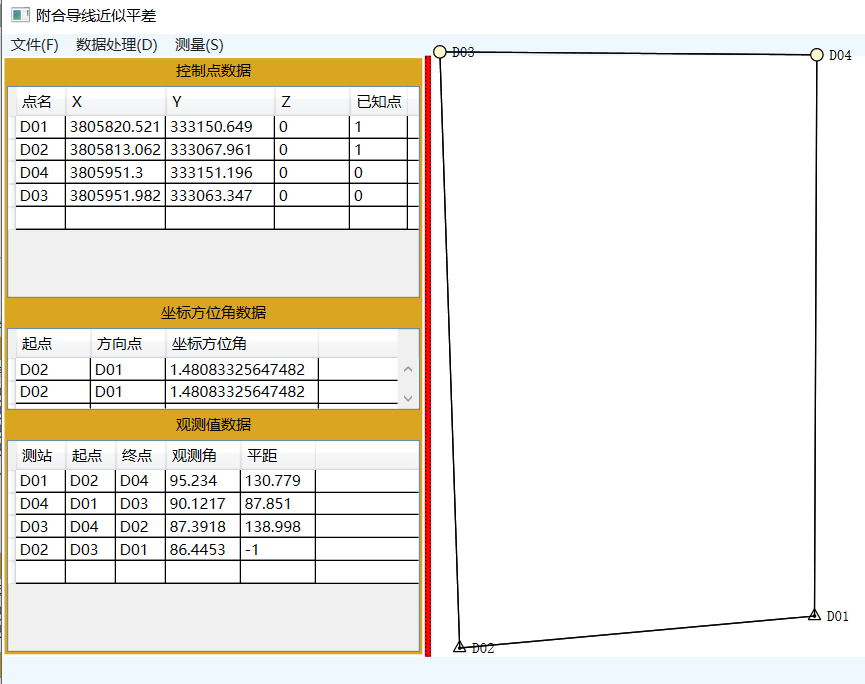
\includegraphics[scale=0.8]{connectingtraverse/ctUI01.png}
	\caption{附合导线界面功能图}
	\label{fig:ctUI01}
\end{figure}

\section{实现代码}

 \begin{lstlisting}[language=xml]
<Window x:Class="SurApp.MainWindow"
xmlns="http://schemas.microsoft.com/winfx/2006/xaml/presentation"
xmlns:x="http://schemas.microsoft.com/winfx/2006/xaml"
xmlns:local="clr-namespace:SurApp.models"
Title="附合导线近似平差" Height="350" Width="525"
WindowState="Maximized">

<DockPanel LastChildFill="True">
<Menu  x:Name="mainmenu" DockPanel.Dock="Top" Background="AliceBlue">
<MenuItem Header="文件(F)">
<MenuItem Header="新建附合导线..." Click="NewMenuItem_Click" />
<MenuItem Header="打开附合导线文件..." Click="OpenMenuItem_Click" />
<MenuItem Header="保存附合导线文件..."  Click="SaveMenuItem_Click" />
<Separator />
<MenuItem Header="导入文本数据" Click="ImportSPointMenuItem_Click"/>
<MenuItem Header="导出文本数据" Click="OutputSPointMenuItem_Click"/>
<Separator />
<MenuItem Header="导出为DXF文件" />
</MenuItem>

<MenuItem Header="数据处理(D)">
<MenuItem Header="附合导线平差" Click="AdjustMenuItem_Click" />
<MenuItem Header="平差成果" Click="AdjustResultMenuItem_Click" />
</MenuItem>

<MenuItem Header="测量(S)">
<MenuItem Header="角度弧度转换" Click="DMS2RADMenuItem_Click" />
<MenuItem Header="坐标方位角计算" Click="AzimuthMenuItem_Click" />
</MenuItem>
</Menu>
<StatusBar x:Name="statusBar" DockPanel.Dock="Bottom" Height="25"  Background="AliceBlue"/>
<Grid>
<Grid.ColumnDefinitions>
<ColumnDefinition Width="75*"/>
<ColumnDefinition Width="5"/>
<ColumnDefinition Width="170*"/>
</Grid.ColumnDefinitions>
<Border BorderThickness="2" Background="Goldenrod" Grid.Column="0">
<Grid x:Name="leftGrid" >
<Grid.RowDefinitions>
<RowDefinition Height="20"/>
<RowDefinition Height="100*"/>
<RowDefinition Height="20"/>
<RowDefinition Height="40*"/>
<RowDefinition Height="20"/>
<RowDefinition Height="100*"/>
</Grid.RowDefinitions>
<TextBlock Text="控制点数据" Grid.Row="0" TextAlignment="Center" Margin="2" />
<DataGrid x:Name="ctrPointDataGrid" Grid.Row="1" AutoGenerateColumns="False" Margin="2" ItemsSource="{Binding CtrPoints}" >
<DataGrid.Columns>
<DataGridTextColumn Header="点名" Binding="{Binding Name}" MinWidth="40"/>
<DataGridTextColumn Header="X" Binding="{Binding X , StringFormat={}{0:##0.###}}" MinWidth="60"/>
<DataGridTextColumn Header="Y" Binding="{Binding Y, StringFormat={}{0:##0.###}}" MinWidth="60" />
<DataGridTextColumn Header="Z" Binding="{Binding Z, StringFormat={}{0:##0.###}}" MinWidth="60"/>
<DataGridTextColumn Header="已知点" Binding="{Binding IsKnown}" MinWidth="30"/>
</DataGrid.Columns>
</DataGrid>

<TextBlock Text="坐标方位角数据" Grid.Row="2" TextAlignment="Center" Margin="2" />
<DataGrid x:Name="azimuthDataGrid" Grid.Row="3" AutoGenerateColumns="False" Margin="2" ItemsSource="{Binding KnownAzimuthes}" >
<DataGrid.Columns>
<DataGridTextColumn Header="起点" Binding="{Binding StartPnt.Name}" MinWidth="60"/>
<DataGridTextColumn Header="方向点" Binding="{Binding EndPnt.Name}" MinWidth="60"/>
<DataGridTextColumn Header="坐标方位角" Binding="{Binding Azimuth}" MinWidth="100" />
</DataGrid.Columns>
</DataGrid>

<TextBlock Text="观测值数据" Grid.Row="4" TextAlignment="Center" Margin="2"/>
<DataGrid x:Name="obsValueDataGrid" Grid.Row="5" AutoGenerateColumns="False"  Margin="2" ItemsSource="{Binding ObsValues}">
<DataGrid.Columns>
<DataGridTextColumn Header="测站" Binding="{Binding StnPnt.Name}" MinWidth="40"/>
<DataGridTextColumn Header="起点" Binding="{Binding StartPnt.Name}" MinWidth="40"/>
<DataGridTextColumn Header="终点" Binding="{Binding EndPnt.Name}" MinWidth="40" />
<DataGridTextColumn Header="观测角" Binding="{Binding DmsAngle}" MinWidth="60"/>
<DataGridTextColumn Header="平距" Binding="{Binding Distance}" MinWidth="60"/>
</DataGrid.Columns>
</DataGrid>

</Grid>
</Border>

<GridSplitter Background="Red" Width="5" Grid.Column="1" HorizontalAlignment="Stretch"/>

<Border BorderThickness="2" Grid.Column="2">
<local:DrawingCanvas x:Name="figureCanvas" SizeChanged="figureCanvas_SizeChanged">
<!--<Canvas.RenderTransform>
<TransformGroup>
<ScaleTransform x:Name="scaleTransform" ScaleX="1" ScaleY="-1" />
<TranslateTransform X ="0"  Y="{Binding ActualHeight, RelativeSource={RelativeSource AncestorType=Canvas}}" />
</TransformGroup>
</Canvas.RenderTransform>-->

<!--<Rectangle Height="50" Width="50" Fill="Red" Stroke="Blue" StrokeThickness="2" Canvas.Left="50" Canvas.Top="50" />

<Rectangle Height="50" Width="50" Fill="#CCCCCCFF" Stroke="Blue" StrokeThickness="2" Canvas.Left="50" Canvas.Top="50" >
<Rectangle.RenderTransform>
<TranslateTransform X="50" Y="50" />
</Rectangle.RenderTransform>
</Rectangle>-->
</local:DrawingCanvas>
</Border>
</Grid>
</DockPanel>

</Window>
 \end{lstlisting}

 \begin{lstlisting}[language=C]
using System;

namespace SurApp.models
{
[Serializable]
public class CtrPoint : ZXY.SPoint
{
private int isKnown = 0;

/// <summary>
/// 是否已知点(0:待定点, 1:已知点)
/// </summary>
public int IsKnown
	{
		get { return isKnown; }
		set
			{
				isKnown = value;
				this.RaisePropertyChange("IsKnown");
			}
	}

public CtrPoint() { }

public CtrPoint(string name, double x, double y, double z, int isKnown) : base(name, x, y, z)
{
		this.isKnown = isKnown;
	}

public override string ToString()
{
return string.Format("{0},{1},{2},{3}", Name, X, Y, Z);
}
}
}

using System;

namespace SurApp.models
{
[Serializable]
public class ObsValue : ZXY.NotificationObject
{
private CtrPoint stnPnt;
public CtrPoint StnPnt
	{
		get { return stnPnt; }
		set
			{
				stnPnt = value;
				this.RaisePropertyChange("StnPnt");
			}
	}

private CtrPoint startPnt;
public CtrPoint StartPnt
	{
		get { return startPnt; }
		set
			{
				startPnt = value;
				this.RaisePropertyChange("StartPnt");
			}
	}

private CtrPoint endPnt;
public CtrPoint EndPnt
	{
		get { return endPnt; }
		set
			{
				endPnt = value;
				this.RaisePropertyChange("EndPnt");
			}
	}

/// <summary>
///  观测角度值(单位:弧度)
/// </summary>
private double angleValue;

/// <summary>
/// 观测角度值(单位:弧度)
/// </summary>
public double AngleValue
	{
		get { return angleValue; }
		set
			{
				angleValue = value;
				this.RaisePropertyChange("DmsAngle");
				this.RaisePropertyChange("AngleValue");
			}
	}

/// <summary>
/// 观测角度值(单位:度分秒)
/// </summary>
public double DmsAngle
	{
		get { return ZXY.SMath.RAD2DMS(angleValue); }
		set
			{
				angleValue = ZXY.SMath.DMS2RAD(value);
				this.RaisePropertyChange("DmsAngle");
				this.RaisePropertyChange("AngleValue");
			}
	}


private double distance;
public double Distance
	{
		get { return distance; }
		set
			{
				distance = value;
				this.RaisePropertyChange("Distance");
			}
	}

public ObsValue() { }

public ObsValue(CtrPoint stnPnt, CtrPoint startPnt, CtrPoint endPnt,
double angleValue, double distance)
{
		this.stnPnt = stnPnt;
		this.startPnt = startPnt;
		this.endPnt = endPnt;
		this.DmsAngle = angleValue;
		this.distance = distance;
	}

private double vB; //角度改正数
public double VB
	{
		get { return vB; }
		set
			{
				vB = value;
				this.RaisePropertyChange("VB");
			}
	}

private double angleV; //改正后角度
public double AngleV
	{
		get { return angleV; }
		set
			{
				angleV = value;
				this.RaisePropertyChange("AngleV");
			}
	}

private double azimuth;
public double Azimuth
	{
		get { return azimuth; }
		set
			{
				azimuth = value;
				this.RaisePropertyChange("Azimuth");
			}
	}

private double dx;
public double DX
	{
		get { return dx; }
		set
			{
				dx = value;
				this.RaisePropertyChange("DX");
			}
	}

private double dy;
public double DY
	{
		get { return dy; }
		set
			{
				dy = value;
				this.RaisePropertyChange("DY");
			}
	}

private double vdx;
public double VDX
	{
		get { return vdx; }
		set
			{
				vdx = value;
				this.RaisePropertyChange("VDX");
			}
	}

private double vdy;
public double VDY
	{
		get { return vdy; }
		set
			{
				vdy = value;
				this.RaisePropertyChange("VDY");
			}
	}

public override string ToString()
{
return string.Format("{0},{1},{2},{3},{4}",
startPnt.Name, startPnt.Name, endPnt.Name,
DmsAngle, distance);
}
}
}

using System;
using System.Collections.Generic;
using System.Collections.ObjectModel;
using System.Windows.Media;
using ZXY;

namespace SurApp.models
{
/// <summary>
/// 用于已知边的坐标方位角信息
/// </summary>
[Serializable]
public class KnownAzimuth : NotificationObject
{
/// <summary>
/// 坐标方位角,单位:弧度
/// </summary>
public double azimuth;
public double Azimuth
	{
		get { return azimuth; }
		set
			{
				azimuth = value;
				this.RaisePropertyChange("Azimuth");
			}
	}

public CtrPoint startPnt; //坐标方位角的起点
public CtrPoint StartPnt
	{
		get { return startPnt; }
		set
			{
				startPnt = value;
				this.RaisePropertyChange("StartPnt");
			}
	}

public CtrPoint endPnt; //坐标方位角的方向点
public CtrPoint EndPnt
	{
		get { return endPnt; }
		set
			{
				endPnt = value;
				this.RaisePropertyChange("EndPnt");
			}
	}

public KnownAzimuth()
{
		startPnt = null;
		endPnt = null;
		azimuth = 0;
	}

public KnownAzimuth(CtrPoint startPnt, CtrPoint endPnt, double az)
{
		this.startPnt = startPnt;
		this.endPnt = endPnt;
		this.azimuth = az;
	}

public override string ToString()
{
if (startPnt == null || endPnt == null) return "~~~";
else
return string.Format("{0},{1},{2}", startPnt.Name, endPnt.Name, ZXY.SMath.RAD2DMS(azimuth));
}
}

[Serializable]
public class CtrNet : NotificationObject
{
private ObservableCollection<KnownAzimuth> knownAzimuthes = new ObservableCollection<KnownAzimuth>();
public ObservableCollection<KnownAzimuth> KnownAzimuthes
	{
		get { return knownAzimuthes; }
	}

private double m0 = 10; //中误差
private double fB;
private double FB; //角度闭合差的限差值
private double fx;
private double fy;
private double fs;

private double sumD;
private double K; // 1/K

//以下定义为绘图使用
private double minX;  //高斯坐标X的最小值xn
private double minY;  //高斯坐标Y的最小值yn
private double maxX; //高斯坐标X的最大值xm
private double maxY; //高斯坐标Y的最大值ym

private double maxVX; //屏幕坐标X的最大值
private double maxVY; //屏幕坐标Y的最大值

private double k;  //变换比例

private ObservableCollection<CtrPoint> ctrPoints =
new ObservableCollection<CtrPoint>();
public ObservableCollection<CtrPoint> CtrPoints
	{
		get { return ctrPoints; }
	}

private ObservableCollection<ObsValue> obsValues =
new ObservableCollection<ObsValue>();
public ObservableCollection<ObsValue> ObsValues
	{
		get { return obsValues; }
	}

/// <summary>
/// 正确的计算路线
/// </summary>
private List<ObsValue> route = new List<ObsValue>();

private bool isDirty = false;

public void ReadDataTextFile(string fileName)
{
using (System.IO.StreamReader sr = new System.IO.StreamReader(fileName))
{
string buffer;

//读入控制点数据
this.ctrPoints.Clear();
while (true)
{
		buffer = sr.ReadLine();
		if (string.IsNullOrEmpty(buffer)) break; //文件末尾或空行退出

		if (buffer[0] == '#') continue;

		string[] its = buffer.Split(new char[1] { ',' });
		if (its.Length != 4) continue; //不为四项控制点数据的继续,直到空行退出

		ctrPoints.Add(new CtrPoint(
		its[0].Trim(), // Name
		double.Parse(its[1]), //X
		double.Parse(its[2]), //Y
		double.Parse(its[3]), //H
		1)); //IsKnown
	}

//读入已知方位角信息:该节有可能不存在,也有可能有一条边,最多两条边
knownAzimuthes.Clear();
while (true)
{
		buffer = sr.ReadLine(); //由于是空行到此,所以继续往下读
		if (buffer == null) break; //文件末尾退出

		if (buffer == "" || buffer[0] == '#') continue; // 略过空行和注释行

		string[] its = buffer.Split(new char[1] { ',' });
		if (its.Length != 3) break; //数据项不为3,可能是角度观测值,退出当前

		KnownAzimuth ka = new KnownAzimuth();

		string ptName = its[0].Trim();
		ka.startPnt = GetCtrPoint(ptName);
		if (ka.startPnt == null)
		{
				ka.startPnt = new CtrPoint(ptName, 0, 0, 0, 0);//非已知点
				this.ctrPoints.Add(ka.startPnt);
			}

		ptName = its[1].Trim();
		ka.endPnt = GetCtrPoint(ptName);
		if (ka.endPnt == null)
		{
				ka.endPnt = new CtrPoint(ptName, 0, 0, 0, 0);//非已知点
				this.ctrPoints.Add(ka.endPnt);
			}

		ka.azimuth = ZXY.SMath.DMS2RAD(double.Parse(its[2]));
		knownAzimuthes.Add(ka);
	}

//读入观测值数据
this.obsValues.Clear();
while (true)
{
//此处可能由上不是3项数据的数据行退出,也有可能是文件末尾到此
//所以得先处理数据,后再读文本数据,否则,容易丢失数据
if (buffer == null) break; //文件末尾到此,继续退出
if (buffer == "" || buffer[0] == '#')//空行或正常的注释略过
{
buffer = sr.ReadLine();
continue;
}

string[] its = buffer.Split(new char[1] { ',' }); //进入正常的数据处理流程
if (its.Length == 5)
{
		string ptName = its[0].Trim();
		CtrPoint stnPnt = GetCtrPoint(ptName);
		if (stnPnt == null)
		{
				stnPnt = new CtrPoint(ptName, 0, 0, 0, 0);//非已知点
				this.ctrPoints.Add(stnPnt);
			}

		ptName = its[1].Trim();
		CtrPoint startPnt = GetCtrPoint(ptName);
		if (startPnt == null)
		{
				startPnt = new CtrPoint(ptName, 0, 0, 0, 0);//非已知点
				this.ctrPoints.Add(startPnt);
			}

		ptName = its[2].Trim();
		CtrPoint endPnt = GetCtrPoint(ptName);
		if (endPnt == null)
		{
				endPnt = new CtrPoint(ptName, 0, 0, 0, 0);//非已知点
				this.ctrPoints.Add(endPnt);
			}

		obsValues.Add(new ObsValue(
		stnPnt, startPnt, endPnt,
		double.Parse(its[3]), //AngleValue
		double.Parse(its[4]))); //Distance
	}

buffer = sr.ReadLine();
}
}
}

public void WriteDataTextFile(string fileName)
{
		using (System.IO.StreamWriter sw = new System.IO.StreamWriter(fileName))
		{
				sw.WriteLine("# Name, X, Y, Z");
				foreach (var pt in this.ctrPoints)
				{
						if(pt.IsKnown == 1) sw.WriteLine( pt );
					}

				sw.WriteLine();
				sw.WriteLine("# StartPnt, EndPnt, Azimuth");
				foreach (var az in this.knownAzimuthes)
				{
						sw.WriteLine( az );
					}

				sw.WriteLine();
				sw.WriteLine("# Station, StartPnt, EndPnt, Angle, Distance");
				foreach (var obs in this.ObsValues)
				{
						sw.WriteLine( obs );
					}
			}
	}


private ObsValue SearchStartObsValue()
{
		/**
		* 搜索起始边,首先:搜索直接给定的坐标方位角
		* 其次:上述搜索不成立的情况,搜索:测站点与后视点均为已知点的观测值
		* 再次:反向搜索:测站点与后视点均为已知点的观测值
		* */
		ObsValue obs = null;

		if (this.knownAzimuthes.Count > 0)
		{
				foreach (var azi in this.knownAzimuthes)
				{
						if (azi.endPnt.IsKnown == 1)
						{
								foreach (var it in obsValues)
								{
										if (it.StartPnt == azi.startPnt && it.StnPnt == azi.endPnt)
										{
												obs = it;
												return obs;
											}
									}
							}
					}
			}
		else if (this.knownAzimuthes.Count == 0)
		{
				foreach (var it in obsValues)
				{
						double az = 0;

						if (it.StartPnt.IsKnown == 1 && it.StnPnt.IsKnown == 1)
						{
								az = ZXY.SMath.Azimuth(it.StartPnt.X, it.StartPnt.Y, it.StnPnt.X, it.StnPnt.Y);
								this.knownAzimuthes.Add(new KnownAzimuth(it.StartPnt, it.StnPnt, az));
								obs = it;
							}

						if (it.StnPnt.IsKnown == 1 && it.EndPnt.IsKnown == 1)
						{
								az = ZXY.SMath.Azimuth(it.StnPnt.X, it.StnPnt.Y, it.EndPnt.X, it.EndPnt.Y);
								this.knownAzimuthes.Add(new KnownAzimuth(it.StnPnt, it.EndPnt, az));
							}
					}
			}
		return obs;
	}


/// <summary>
/// 递归搜索观测值obs0的下一条边
/// </summary>
/// <param name="obs0">当前观测值</param>
/// <returns>1:附合导线, -1:不构成附合导线</returns>
private int SearchObsValue(ObsValue obs0)
{
//传进来的第一条边应为起始边
ObsValue obsi = null;

foreach (var it in obsValues)
{
if (it == obs0) continue;

if (obs0.StnPnt == it.StartPnt && obs0.EndPnt == it.StnPnt)  //满足条件的下一条边
{
obsi = it;
break;
}
}

if (obsi == null) return -1;//没找到这样的边

this.route.Add(obsi);
if (obsi.StnPnt.IsKnown == 1 && obsi.EndPnt.IsKnown == 1) //附合到另一条已知边了,退出
{
return 1;
}
else
SearchObsValue(obsi); //递归继续寻找下一条这样的边

return 0;
}


/// <summary>
/// 搜索正确的计算路线
/// </summary>
/// <returns>是否成功</returns>
public bool SearchCalRoute()
{
		ObsValue obs0 = SearchStartObsValue();
		if (obs0 == null) return false;

		route.Clear(); //清空搜索线路

		route.Add(obs0);
		SearchObsValue(obs0);
		return true;
	}

/// <summary>
/// 简易平差
/// </summary>
/// <returns>0:成功</returns>
public int Adjust()
{
		/*
		1. 求起始边: 后视->测站 的方位角
		求末边:测站->前视 的方位角
		2. 计算角度闭合差fB,FB
		3. 改正角度值
		4. 推算各边坐标方位角
		5. 计算各边的坐标增量
		6.计算fx, fy, fs, 1/K
		7.计算改正后的坐标增量
		8.计算各点的坐标值
		*/
		if (this.obsValues.Count == 0) return -1; //观测值为空

		if (SearchCalRoute() == false) return -2; //搜索不到正确的附合路线

		double az0 = this.knownAzimuthes[0].azimuth;
		CtrPoint startPnt0 = this.knownAzimuthes[0].startPnt;
		CtrPoint stnPnt0 = this.knownAzimuthes[0].endPnt;

		double azn = this.knownAzimuthes[1].azimuth;
		CtrPoint stnPntn = this.knownAzimuthes[1].startPnt;
		CtrPoint endPntn = this.knownAzimuthes[1].endPnt;

		double azi = az0;
		double n = route.Count;
		foreach (var obs in route) //foreach (var obs in this.ObsValues)
		{
				obs.Azimuth = azi + obs.AngleValue + Math.PI;
				if (obs.Azimuth >= 2 * Math.PI) obs.Azimuth -= 2 * Math.PI;
				if (obs.Azimuth < 0) obs.Azimuth += 2 * Math.PI;

				azi = obs.Azimuth;
			}

		fB = azi - azn; //单位:弧度
		FB = m0 * 2 * Math.Sqrt(n); //单位:秒

		//改正角度,推算各边改正后的方位角
		azi = az0;
		double vi = -fB / n;
		foreach (var obs in route) //foreach (var obs in this.ObsValues)
		{
				obs.VB = vi;
				obs.AngleV = obs.AngleValue + obs.VB;
				obs.Azimuth = azi + obs.AngleV + Math.PI;
				if (obs.Azimuth >= 2 * Math.PI) obs.Azimuth -= 2 * Math.PI;
				if (obs.Azimuth < 0) obs.Azimuth += 2 * Math.PI;
				azi = obs.Azimuth;
			}

		//计算各边的坐标增量
		double sumDX = 0, sumDY = 0;
		sumD = 0;
		foreach (var obs in route) //foreach (var obs in this.ObsValues)
		{
				if (obs.Distance <= 0) continue;

				obs.DX = obs.Distance * Math.Cos(obs.Azimuth);
				obs.DY = obs.Distance * Math.Sin(obs.Azimuth);
				sumDX += obs.DX;
				sumDY += obs.DY;
				sumD += obs.Distance;
			}
		fx = stnPnt0.X + sumDX - stnPntn.X;
		fy = stnPnt0.Y + sumDY - stnPntn.Y;
		fs = Math.Sqrt(fx * fx + fy * fy);
		K = sumD / fs;

		//改正坐标增量,计算各点坐标
		foreach (var obs in route) //foreach (var obs in this.ObsValues)
		{
				if (obs.Distance <= 0) continue;

				obs.VDX = -fx / sumD * obs.Distance;
				obs.VDY = -fy / sumD * obs.Distance;

				obs.EndPnt.X = obs.StnPnt.X + obs.DX + obs.VDX;
				obs.EndPnt.Y = obs.StnPnt.Y + obs.DY + obs.VDY;
			}

		return 0;
	}

private CtrPoint GetCtrPoint(string pointName)
{
		foreach (var pt in this.ctrPoints)
		{
				if (pt.Name == pointName)
				return pt;
			}

		return null;
	}

public void OnDraw(DrawingCanvas canvas)
{
		if (this.ctrPoints.Count < 1) return;

		GetGaussXySize();

		maxVX = canvas.ActualWidth-20;
		maxVY = canvas.ActualHeight;

		double kx = maxVX / (maxY - minY);
		double ky = maxVY / (maxX - minX);
		k = kx <= ky ? kx : ky;

		canvas.ClearAll(); //先清除屏幕

		//画观测值
		double x0, y0, x1, y1, x2, y2; //画直线的两个端点
		foreach (var it in this.obsValues)
		{
				if (it.StnPnt.X <= 0 && it.StnPnt.Y <= 0) continue; //略过坐标为0的点
				GaussXyToViewXy(it.StnPnt.X, it.StnPnt.Y, out x0, out y0);

				if (it.StartPnt.X > 0 && it.StartPnt.Y > 0)
				{
						GaussXyToViewXy(it.StartPnt.X, it.StartPnt.Y, out x1, out y1);
						canvas.DrawLine(x1, y1, x0, y0, Brushes.Black, 1);
					}

				if (it.EndPnt.X > 0 && it.EndPnt.Y > 0)
				{
						GaussXyToViewXy(it.EndPnt.X, it.EndPnt.Y, out x2, out y2);
						canvas.DrawLine(x0, y0, x2, y2, Brushes.Black, 1);
					}
			}

		//再画控制点
		foreach (var pt in this.ctrPoints)
		{
				if (pt.X <= 0 && pt.Y <= 0) continue; //排除坐标为0的点

				GaussXyToViewXy(pt.X, pt.Y, out x0, out y0);
				if(pt.IsKnown == 1)
				canvas.DrawKnCtrPnt(x0, y0, Brushes.Black, 1);
				else
				canvas.DrawCtrPnt(x0, y0, Brushes.Black, 1);
				canvas.DrawText(pt.Name, x0 + 10, y0 - 7);
			}
	}

private void GaussXyToViewXy(double xt, double yt, out double xp, out double yp)
{
		//xp = x0 + kx(yt - yn);
		//yp = y1 - (y0 + ky * (xt - xn));
		// x0 = y0 =0 且 kx = ky =k, 故以上公式简化为:

		xp = 5 + k * (yt - minY); //x0 = 5;
		yp = maxVY - (5 + k * (xt - minX)); //y0=5;
	}

private void GetGaussXySize()
{
minX = this.ctrPoints[0].X; minY = this.ctrPoints[0].Y;
maxX = this.ctrPoints[0].X; maxY = this.ctrPoints[0].Y;

for (int i = 1; i < this.ctrPoints.Count; i++) //如果只有一个点,由循环条件知,不会执行循环体
{
if (this.ctrPoints[i].X <= 0 && this.ctrPoints[i].Y <= 0) continue;

if (this.ctrPoints[i].X < minX) minX = this.ctrPoints[i].X;
if (this.ctrPoints[i].Y < minY) minY = this.ctrPoints[i].Y;

if (this.ctrPoints[i].X > maxX) maxX = this.ctrPoints[i].X;
if (this.ctrPoints[i].Y > maxY) maxY = this.ctrPoints[i].Y;
}

//针对一个点或点范围较小的情况,进行范围扩展
if (minX + 10 > maxX) { maxX = minX + 10; minX = maxX - 20; }
if (minY + 10 > maxY) { maxY = minY + 10; minY = maxY - 20; }
}
}
}

using System.Globalization;
using System.Windows;
using System.Windows.Media;

namespace SurApp.models
	{
		public class DrawingCanvas : System.Windows.Controls.Canvas
			{
				private VisualCollection visuals;

				public DrawingCanvas()
				{
						visuals = new VisualCollection(this);
					}

				//获取Visual的个数
				protected override int VisualChildrenCount
					{
						get { return visuals.Count; }
					}

				//获取Visual
				protected override Visual GetVisualChild(int index)
				{
						return visuals[index];
					}

				//添加Visual
				public void AddVisual(Visual visualObject)
				{
						visuals.Add( visualObject );
					}

				//删除Visual
				public void RemoveVisual(Visual visualObject)
				{
						base.RemoveLogicalChild(visualObject);
					}

				//命中测试
				public DrawingVisual GetVisual(System.Windows.Point point)
				{
						HitTestResult hitResult = VisualTreeHelper.HitTest(this, point);
						return hitResult.VisualHit as DrawingVisual;
					}

				public void ClearAll()
				{
						this.visuals.Clear();
					}


				//使用DrawVisual画Polyline
				public void DrawLine(double x0, double y0, double x1, double y1,  Brush color, double thinkness)
				{
						DrawingVisual visualLine = new DrawingVisual();
						DrawingContext dc = visualLine.RenderOpen();
						Pen pen = new Pen(color, thinkness);
						pen.Freeze();  //冻结画笔,这样能加快绘图速度
						dc.DrawLine(pen, new Point(x0, y0),  new Point(x1, y1) );

						dc.Close();
						visuals.Add(visualLine);
					}

				public void DrawText(string text, double x, double y)
				{
						DrawingVisual visualText = new DrawingVisual();
						DrawingContext dc = visualText.RenderOpen();
						Typeface tp = new Typeface(new FontFamily("宋体"), FontStyles.Normal, FontWeights.Normal, FontStretches.Normal);
						FormattedText ft = new FormattedText(text, CultureInfo.CurrentCulture,
						FlowDirection.LeftToRight, tp, 12, Brushes.Black);
						dc.DrawText(ft, new Point(x, y) );
						dc.Close();
						visuals.Add( visualText );
					}

				//使用DrawVisual画Circle,用作控制点
				public void DrawCtrPnt(double x, double y,  Brush color, double thinkness)
				{
						DrawingVisual visualCircle = new DrawingVisual();
						DrawingContext dc = visualCircle.RenderOpen();
						Pen pen = new Pen(color, thinkness);
						pen.Freeze();  //冻结画笔,这样能加快绘图速度
						dc.DrawEllipse(Brushes.LemonChiffon,  pen,  new Point(x, y),  5, 5);
						dc.Close();
						visuals.Add(visualCircle);
					}

				//使用DrawVisual画Circle,用作控制点
				public void DrawKnCtrPnt(double x, double y, Brush color, double thinkness)
				{
						DrawingVisual visualCircle = new DrawingVisual();
						DrawingContext dc = visualCircle.RenderOpen();
						Pen pen = new Pen(color, thinkness);
						pen.Freeze();  //冻结画笔,这样能加快绘图速度
						dc.DrawEllipse(Brushes.Black, pen, new Point(x, y), 1, 1);
						dc.DrawLine(pen, new Point(x-5, y+2.9), new Point(x+5, y+2.9));
						dc.DrawLine(pen, new Point(x + 5, y + 2.9), new Point(x, y - 5.8));
						dc.DrawLine(pen, new Point(x, y - 5.8), new Point(x - 5, y + 2.9));
						dc.Close();
						visuals.Add(visualCircle);
					}
			}
	}

 \end{lstlisting}
 %%附合导线近似平差程序设计
%!TEX root = ../clcxsj.tex

\chapter{高斯投影正反算与换带}

高斯投影是为解决球面与平面之间的坐标映射问题,即大地坐标(B,
L)与高斯平面直角坐标$(x,y)$之间的相互换算,以及不同带之间的高斯坐标
的换算问题。

本章将运用$C\#$编程语言编写一个通用的高斯投影程序,用于1954北京坐标系、1980西安坐标系、
WGS84坐标系以及CGCS2000大地坐标系或自定义参考椭球的高斯投影正反算与换带计算。


\section{高斯投影的数学模型}

为了编制正确而且高效的高斯投影与换带程序,我们首先需要分析高斯投影的数学模型,也就是我们
常说的算法。

本章所引用的公式来自:
孔祥元,郭际明,刘宗泉.大地测量学基础-2版.武汉:武汉大学出版社,2010.5,
以下将这本书简称为大地测量学基础或大地测量学。

高斯投影是在椭球的几何参数(长半轴a、短半轴b、扁率$\alpha$)确定的条件下,根据
给定的数学模型来进行计算的,我们首先分析这些计算公式与数学模型。

\begin{enumerate}

\item 基本公式

\begin{enumerate}
\item 扁率:
$$\alpha=\frac{a-b}{a}$$

\item 第一偏心率:
$$e=\sqrt{\frac{a^2-b^2}{a^2}}$$

\item 第二偏心率:
$$e'=\sqrt{\frac{a^{2}-b^{2}}{b^{2}}}$$

\item 子午圈曲率半径:
$$M=\frac{a(1-e^2)}{(1-e^2\sin ^2 B)^{\frac{3}{2}}}$$

\item 卯酉圈曲率半径:
$$N=\frac{a}{\sqrt{1-e^2\sin^2 B}}$$

\item 辅助符号:
$$t=\tan B\qquad\eta=e'\cos B$$
\end{enumerate}

\item 椭球面梯形图幅面积计算

$$P = \frac{b^2}{2}(L_2 - L_1) \left | \frac{\sin B}{1-e^2\sin^2 B} + \frac{1}{2e}\ln \frac{1+e\sin B}{1-e\sin B}\right |_{B1} ^{B2} $$
公式引用自《大地测量学基础》第121页(4-140)。

$$P=b^2(L_2 - L_1) \left | sinB + \frac{2}{3}e^2 \sin ^3 B + \frac{3}{5}e^4 \sin^5 B + \frac{4}{7}e^6 \sin ^7 B \right | _{B_1} ^{B_2}$$

公式引用自《大地测量学基础》第121页(4-142),该公式为(4-140)的展开式。

\item 子午线弧长
\begin{equation}
X=a_0 B - \frac{a_2}{2}\sin 2B + \frac{a_4}{4}\sin 4B
- \frac{a_6}{6} \sin 6B  + \frac{a_8}{8}\sin 8B
\end{equation}

式中:
\begin{equation}
\left  . \begin{aligned}
a_0 &= m_0 + \frac{m_2}{2} + \frac{3}{8}m_4 + \frac{5}{16}m_6 + \frac{35}{128}m_8  \\
a_2 &= \frac{m_2}{2} + \frac{m_4}{2} + \frac{15}{32}m_6 + \frac{7}{16}m_8  \\
a_4 &= \frac{m_4}{8} + \frac{3}{16}m_6 + \frac{7}{32}m_8  \\
a_6 &= \frac{m_6}{32} + \frac{m_8}{16}  \\
a_8 &= \frac{m_8}{128}
\end{aligned} \right \}
\end{equation}

式中$m_0, m_2, m_4, m_6, m_8$的值为:

\begin{equation}
\left . 
\begin{aligned}
m_0 &= a(1-e^2) \\
m_2 &= \frac{3}{2}e^2 m_0  \\
m_4 &= \frac{5}{4}e^2 m_2   \\
m_6 &= \frac{7}{6}e^2 m_4   \\
m_8 &= \frac{9}{8}e^2 m_6
\end{aligned} 
\right \}
\end{equation}

公式引用自《大地测量学基础》第115页(4-101)、(4-100)与(4-72).

或用很多书上都引用的公式:

\begin{equation}
X=c[\beta_0 B + (\beta_2 \cos B + \beta_4 \cos^3 B + \beta_6 \cos^5 B + \beta_8 \cos^7 B) \sin B] 
\end{equation}

式中 c 为极曲率半径,其值为: $c= a^2 / b$,
$\beta_0, \beta_2, \beta_4, \beta_6, \beta_8$的值为:

\begin{equation}
\left .
\begin{aligned}
\beta_0 &= 1 - \frac{3}{4}e'^2 + \frac{45}{64}e'^4 - \frac{175}{256}e'^6 + \frac{11025}{16384}e'^8  \\
\beta_2 &= \beta_0 -1  \\
\beta_4 &= \frac{15}{32}e'^4 - \frac{175}{384}e'^6 + \frac{3675}{8192}e'^8   \\
\beta_6 &= -\frac{35}{96}e'^6 + \frac{735}{2048}e'^8   \\
\beta_8 &= \frac{315}{1024}e'^8
\end{aligned} 
\right \}
\end{equation}

公式引用自《大地测量学基础》第115页(4-107)、与(4-108)。

或用以下公式:

\begin{equation}
X=d [\alpha_0 B  - ( \alpha_2 \sin B + \alpha_4 \sin ^3 B + \alpha_6 \sin ^5 B + \alpha_8 \sin^7 ) \cos B]
\end{equation}

式中 d 为赤道子午曲率半径, 其值为 $d=b^2 / a $, 
$\alpha_0, \alpha_2, \alpha_4, \alpha_6, \alpha_8$的值为:

\begin{equation}
\left .
\begin{aligned}
\alpha_0 &= 1+\frac{3}{4}e^2+\frac{45}{64}e^4+\frac{175}{256}e^6+\frac{11025}{16384}e^8  \\
\alpha_2 &= \alpha_0 - 1 \\
\alpha_4 &= \frac{15}{32}e^4+\frac{175}{384}e^6+\frac{3675}{8192}e^8 \\
\alpha_6 &= \frac{35}{96}e^6+\frac{735}{2048}e^8 \\
\alpha_8 &= \frac{315}{1024}e^8
\end{aligned} 
\right \}
\end{equation}

\item 坐标正算
\begin{equation}
\left .
\begin{aligned}
x&=X+\frac{N}{2}sinBcosBl^2 +\frac{N}{24}sinBcos^3B(5-t^2 +9\eta^2+4\eta^4)l^4 \\
  &+\frac{N}{720}sinBcos^5 B(61-58t^2 +t^4)l^6  \\
y&=NcosBl+\frac{N}{6}cos^3 B(1-t^2 +\eta^2 )l^3 \\
        &+\frac{N}{120}cos^5 B (5-18t^2+t^4 +14\eta^2 -58\eta^2t^2)l^5
\end{aligned}
 \right \}
\end{equation}

公式引用自《大地测量学基础》第169页(4-367)。

\item 坐标反算

\begin{equation}
\left  .
\begin{aligned}
B&=B_f - \frac{t_f}{2M_f N_f }y^2 +\frac{t_f}{24 M_f N_f ^3}
(5 + 3t_f ^2  + \eta_f ^2 - 9\eta_f ^2 t_f^2)y^4 \\
 &- \frac{t_f}{720 M_f N_f ^5}(61 + 90t_f ^2 + 45t_f ^4)y^6 \\
l&=\frac{1}{N_f cosB_f}y - \frac{1}{6N_f ^3 cosB_f}(1 + 2t_f ^2 + \eta_f ^2)y^3  \\
 &+ \frac{1}{120N_f ^5 cosB_f}(5 + 28t_f ^2 + 24t_f ^4 + 6\eta_f ^2 +8\eta_f ^2 t_f ^2)y^5
\end{aligned} 
\right \}
\end{equation}

公式引用自《大地测量学基础》第171页(4-383)。


\item 平面子午线收敛角计算

利用$(B, l)$计算公式如下:
$$\gamma = \sin B \cdot l + \frac{1 + 3 \eta^2 + 2 \eta^4}{3} \sin B \cos ^2 B \cdot l^3
+ \frac{2 - t^2}{15}\sin B \cos ^4 B \cdot l^5$$

公式引用自《大地测量学基础》第181页(4-408)。

利用$(x, y)$计算公式如下:

$$\gamma = \frac{1}{N_f}t_f y - \frac{1+t_f ^2 - \eta_f ^2}{3N_f ^3}t_f y^3
+ \frac{2+5t_f^2+3t_f^4}{15N_f ^5}t_fy^5$$

公式引用自《大地测量学基础》第182页(4-410)。

\item 长度比计算

利用$(B, l)$计算公式如下:
$$m=1+\frac{1}{2}l^2 \cos ^2 B(1+\eta^2) + \frac{1}{24}l^4\cos ^4 B(5-4t^2)$$

公式引用自《大地测量学基础》第189页(4-447)。

利用$(x, y)$计算公式如下:

$$m=1+\frac{y^2}{2R^2} + \frac{y^4}{24R^4}$$

式中$R=\sqrt{MN}$,公式引用自《大地测量学基础》第189页(4-451)。

\end{enumerate}

\section{程序功能分析与设计}

\subsection{高斯投影的主要内容}
\begin{enumerate}
    \item 坐标正算:将点的大地坐标转换成高斯投影平面直角坐标。
    \item 坐标反算:将点的高斯投影平面直角坐标转换成大地坐标。
    \item 换带计算:将某带的点的高斯投影平面直角坐标转换成邻带或某中央
    子午线经度的高斯投影平面直角坐标。
    \item 其他计算:计算子午线收敛角、长度比等。
\end{enumerate}

\subsection{参考椭球类的设计}

分析以上各个计算公式发现,如果椭球长半轴与扁率确定,参考椭球的第一偏心率$e$、
第二偏心率$e'$,子午线弧长计算的辅助计算参数$(m_0, m_2, m_4, m_6, m_8)$与
$(a_0, a_2, a_4, a_6, a_8)$也就确定了,其中的$(m_0, m_2, m_4, m_6, m_8)$
作为计算$(a_0, a_2, a_4, a_6, a_8)$的值使用过一次。也就是说这些参数对于某一种确定的
参考椭球是常数。而$(M,N,t,\eta)$则是纬度$B$的函数。

我们新建一 WPF 项目,命名为GaussProj,程序中我们将应用WPF技术编写图形界面。

在高斯投影中由于要处理角度与点等数据,我们可以将前面的角度处理函数DMS2RAD与RAD2DMS与SPoint点类
拷贝到当前项目中来,也可以将其打包成一 Class Library(.NET Framework)即类库文件引用到当前项目中,
在当前项目中尽量不修改前面的各个功能代码。

基于上一小节的分析,我们新建一椭球类$(Spheroid)$,在其中我们定义以上与椭球类型
相关的元素。代码如下所示:

\begin{lstlisting}[language=C]
namespace GaussProj
{
    /// <summary>
    /// 参考椭球
    /// </summary>
    public class Spheroid
    {
        /// <summary>
        /// 长半轴
        /// </summary>
        public double a { get; set; }

        /// <summary>
        /// 短半轴
        /// </summary>
        public double b { get; set; }

        /// <summary>
        /// 扁率分母
        /// </summary>
        public double f { get; set; }  //(a-b)/a = 1/f

        /// <summary>
        /// 第一偏心率的平方
        /// </summary>
        public double e2 { get; set; }

         /// <summary>
        /// 第二偏心率的平方
        /// </summary>
        public double eT2 { get; set; }

        //计算子午线弧长时的各个系数项
        private double a0;
        private double a2;
        private double a4;
        private double a6;
        private double a8;
    }
}
\end{lstlisting}

在各项计算中,第一偏心率与第二偏心率的直接使用较少,其平方值用的较多,因此在
Spheroid类我们直接用其平方值。

 在Spheroid类中我们可以如下直接定义构造函数用于初始化其各个字段(Field):
  \begin{lstlisting}[language=C]
/// <summary>
/// 构造函数
/// </summary>
private Spheroid(double semimajor_axis, double inverse_flattening)
{
    this.a = semimajor;
    this.f =  inverse_flattening;
    ...................................................
}
\end{lstlisting}

但这样我们可能无法为已知的一些参考椭球直接提供参数,所以我们将构造函数定义
为 private,让用户无法通过new直接创建实例化对象。我们设计类的静态函数
Create**** 来创建类Spheroid的实例化对象,其代码如下:

 \begin{lstlisting}[language=C]
/// <summary>
/// 构造函数
/// </summary>
private Spheroid(){}

/// <summary>
/// 初始化椭球参数的内部函数
/// </summary>
private void Init(double semimajor_axis, double inverse_flattening)
{
    this.a = semimajor_axis; this.f = inverse_flattening;
    b = a * (1 - 1 / f);

    e2 = 1 - b / a * b / a;
    eT2 = a / b * a / b - 1;

    double m0 = a * (1 - e2);
    double m2 = 3.0 / 2.0 * e2 * m0;
    double m4 = 5.0 / 4.0 * e2 * m2;
    double m6 = 7.0 / 6.0 * e2 * m4;
    double m8 = 9.0 / 8.0 * e2 * m6;

    a0 = m0 + m2 / 2.0 + 3.0 / 8.0 * m4 + 5.0 / 16.0 * m6
                  + 35.0 / 128.0 * m8;
    a2 = m2 / 2.0 + m4 / 2.0 + 15.0 / 32.0 * m6 + 7.0 / 16.0 * m8;
    a4 = m4 / 8.0 + 3.0 / 16.0 * m6 + 7.0 / 32.0 * m8;
    a6 = m6 / 32.0 + m8 / 16.0;
    a8 = m8 / 128.0;
}

public static Spheroid CreateBeiJing1954()
{
    Spheroid spheroid = new Spheroid();
    spheroid.Init(6378245, 298.3);
    return spheroid;
}

public static Spheroid CreateXian1980()
{
    Spheroid spheroid = new Spheroid();
    spheroid.Init(6378140, 298.257);
    return spheroid;
}

public static Spheroid CreateWGS1984()
{
    Spheroid spheroid = new Spheroid();
    spheroid.Init(6378137, 298.257223563);
    return spheroid;
}

public static Spheroid CreateCGCS2000()
{
    Spheroid spheroid = new Spheroid();
    spheroid.Init(6378137, 298.257222101);
    return spheroid;
}

public static Spheroid CreateCoordinateSystem(double semimajor_axis,
      double inverse_flattening)
{
    Spheroid spheroid = new Spheroid();
    spheroid.Init(semimajor_axis, inverse_flattening);
    return spheroid;
}
\end{lstlisting}

这种将构造函数设为private,通过静态函数来创建实例化对象的技术在软件设计中
会经常用到。同时在设计类的方法时,应注意访问权限的设置,如上面代码中Init函数,
在类中用于初始化椭球的各项几何参数,并不需要在类外来调用它,所以我们将其设置为
private权限。

\subsection{高斯投影正算功能的实现}
有了类Spheroid的设计,我们先来完成高斯投影正算功能。
为了避免在计算中频繁的进行度分秒与弧度之间的转换问题,
我们设定除了特别声明之外,在类Spheroid中所用的角度均为弧度。

我们将高斯投影正算的函数名称定义为 BLtoXY,其设计如下:

\begin{lstlisting}[language=C]
/// <summary>
/// 高斯投影正算
/// </summary>
/// <param name="B">纬度,单位:弧度</param>
/// <param name="L">经度,单位:弧度</param>
/// <param name="L0">中央子午线经度,单位:弧度</param>
/// <param name="x">高斯平面x坐标</param>
/// <param name="y">高斯平面y坐标</param>
public void BLtoXY(double B, double L, double L0,
    out double x, out double y)
{
    ......................................
}
\end{lstlisting}

由于函数的返回值为两个值x与y,无法以函数的返回值return的形式返回计算结果,
所以我们用函数参数 out 的形式将计算结果返回。

 由前面的高斯投影正算公式分析可知,高斯投影正算的计算较为简单,没有复杂的逻辑,
 先计算经差,然后计算子午线弧长后就可以直接写计算坐标x,y的算法了。
 但公式较为复杂,极容易写错,公式中具有大量的平方、四次方等变量。因此在编程时
 应将这些变量命名为与其相似的形式并提前计算。相关代码如下:

\begin{lstlisting}[language=C]
/// <summary>
/// 计算子午线弧长
/// </summary>
/// <param name="B">纬度(单位:弧度)</param>
/// <returns>子午线弧长</returns>
private double funX(double B)
{
    return a0 * B - a2 / 2.0 * Math.Sin(2 * B)
        + a4 / 4.0 * Math.Sin(4 * B)
        - a6 / 6.0 * Math.Sin(6 * B)
        + a8 / 8.0 * Math.Sin(8 * B);
}

private double funN(double sinB)
{
    return a / Math.Sqrt(1 - e2 * sinB * sinB);
}

/// <summary>
/// 高斯投影正算
/// </summary>
/// <param name="B">纬度,单位:弧度</param>
/// <param name="L">经度,单位:弧度</param>
/// <param name="L0">中央子午线经度,单位:弧度</param>
/// <param name="x">高斯平面x坐标</param>
/// <param name="y">高斯平面y坐标</param>
public void BLtoXY(double B, double L, double L0,
    out double x, out double y)
{
    double l = L - L0; //计算经差

    double sinB = Math.Sin(B);
    double cosB = Math.Cos(B);
    double cosB2 = cosB * cosB;
    double cosB4 = cosB2 * cosB2;
    double t = Math.Tan(B);
    double t2 = t * t;
    double t4 = t2 * t2;
    double g2 = eT2 * cosB * cosB;
    double g4 = g2 * g2;
    double l2 = l * l;
    double l4 = l2 * l2;

    double X = funX(B); //计算子午线弧长
    double N = funN(sinB);

    x = X + 0.5 * N * sinB * cosB * l2 * (1
        + cosB2 / 12.0 * (5 - t2 + 9 * g2 + 4 * g4) * l2
        + cosB4 / 360.0 * (61 - 58 * t2 + t4) * l4);


   y = N * cosB * l * (1
        + cosB2 * (1 - t2 + g2) * l2 / 6.0
        + cosB4 * (5 - 18 * t2 + t4 + 14 * g2 - 58 * g2 * t2)
                * l4 / 120.0);
}
\end{lstlisting}

利用 BLtoXY 函数就可以进行高斯投影正算了,其算法流程为:

\begin{lstlisting}[language=C]
//创建克拉索夫斯基参考椭球
Spheroid  spheroid = Spheroid.CreateBeiJing1954();

//传入点的纬度B、经度与中央子午线经度,单位为弧度
double B = ZXY.SMath.DMS2RAD(21.58470845);
double L = ZXY.SMath.DMS2RAD(113.25314880);
double L0 = ZXY.SMath.DMS2RAD(111);
double x, y;

spheroid.BLtoXY(B, L, L0, out x, out y);
\end{lstlisting}

点的纬度、经度为:$ B = 21 \degree 58'47.0845'',  L= 113\degree 25'31.4880''$,
中央子午线经度为:$L0 = 111\degree$,
计算出的坐标为:$x=2433586.692, y=250547.403$, 坐标y为点的自然坐标,
未加常数500km与带号。

\subsection{高斯投影反算功能的实现}
由高斯投影反算公式分析,在反算时需要首先计算底点纬度。底点纬度需要由
子午线弧长公式进行反算,由该公式可以看出,已知X=x时,这个函数在计算B值时它
并不是一个线型函数,不能直接计算。解决这类问题的计算方法就是迭代计算,我们将公式
进行变换,如下所示:

$$B= (X + \frac{a_2}{2}\sin 2B - \frac{a_4}{4}\sin 4B
+ \frac{a_6}{6} \sin 6B  - \frac{a_8}{8}\sin 8B)/a_0$$

在该公式中,两边都有B,我们将公式右边的B赋初始值$B_0=X/a_0$代入可以
计算出新的$B$值,循环进行计算,由于该迭代收敛,两值之差 $B - B_0$ 在一定范围内时
我们认为其值 $B$ 即为我们的解。

因此底点纬度计算函数设计为:

\begin{lstlisting}[language=C]
/// <summary>
/// 计算底点纬度
/// </summary>
/// <param name="x">高斯平面坐标x</param>
/// <returns>底点纬度</returns>
private double funBf(double x)
{
    double sinB, sin2B, sin4B, sin6B, sin8B;
    double Bf0 = x / a0, Bf = 0; //子午线弧长的初值
    int i = 0;
    while (i < 10000)//设定最大迭代次数
    {
        sinB = Math.Sin(Bf0);
        sin2B = Math.Sin(2 * Bf0);
        sin4B = Math.Sin(4 * Bf0);
        sin6B = Math.Sin(6 * Bf0);
        sin8B = Math.Sin(8 * Bf0);
        Bf = (x
        + a2 * sin2B / 2
        - a4 * sin4B / 4
        + a6 * sin6B / 6
        - a8 * sin8B / 8) / a0;

        if (Math.Abs(Bf - Bf0) < 1e-10) //计算精度
            return Bf;
        else
        {
            Bf0 = Bf;
            i++;
        }
    }
    return -1e12;
}
\end{lstlisting}

 在底点纬度计算出以后,高斯投影反算计算就没有难度了。
 我们将函数名命名为 XYtoBL,其函数设计为:
 \begin{lstlisting}[language=C]
public void XYtoBL(double x, double y, double L0,
    out double B, out double L)
{
   double Bf = funBf(x);

    double cosBf = Math.Cos(Bf);
    double gf2 = eT2 * cosBf * cosBf;
    double gf4 = gf2 * gf2;
    double tf = Math.Tan(Bf);
    double tf2 = tf * tf;
    double tf4 = tf2 * tf2;
    double sinB = Math.Sin(Bf);
    double Nf = funN(sinB);
    double Mf = funM(sinB);
    double Nf2 = Nf * Nf;
    double Nf4 = Nf2 * Nf2;
    double y2 = y * y;
    double y4 = y2 * y2;

    B = Bf + tf * y2 / Mf / Nf * 0.5 * (
       -1.0
      + y2 * (5.0 + 3.0 * tf2 + gf2 - 9.0 * gf2 * tf2) / 12.0 / Nf2
      - y4 * (61.0 + 90.0 * tf2 + 45.0 * tf4) / 360.0 / Nf4);

   double l = y / Nf / cosBf * (
        1.0
      - y2 / 6.0 / Nf2 * (1.0 + 2.0 * tf2 + gf2)
     + y4 / 120.0 / Nf4
     * (5.0 + 28.0 * tf2 + 24.0 * tf4 + 6.0 * gf2 + 8.0 * gf2 * tf2));

    L = L0 + l;
}
\end{lstlisting}

该函数中还有Nf与Mf需要计算,Nf的计算同前面的funN函数,Mf的计算函数为
 \begin{lstlisting}[language=C]
private double funM(double sinB)
{
    return a * (1 - e2) * Math.Pow(1 - e2 * sinB * sinB, -1.5);
}
\end{lstlisting}

 有了高斯投影反算函数 XYtoBL, 就可以比较容易的写出其反算示例了,如以下代码所示:

\begin{lstlisting}[language=C]
//创建克拉索夫斯基参考椭球
Spheroid  spheroid = Spheroid.CreateBeiJing1954();

//传入点的X、Y坐标与中央子午线经度(单位为弧度)
double x=2433586.692, y=250547.403;
double L0 = ZXY.SMath.DMS2RAD(111);

double B, L;
spheroid.XYtoBL(x, y, L0, out B, out L);
//B= ZXY.SMath.RAD2DMS(B);
//L= ZXY.SMath.RAD2DMS(L);
\end{lstlisting}

传入的y坐标应为真实坐标值,应不包括500km与带号等。
如果计算的经纬度需向界面展示,还应像上述代码后两行所示将其值转换为
度分秒形式。

计算出的点的纬度与经度为:
$B=21 \degree 58'47.0845'', L=113\degree 25'31.4880''$

计算点的子午线收敛角与计算某点处的长度变形值均比较简单,可以在正算或反算时将其同时
计算出,大家可以自己练习完成,在此就不再讲述了。

\subsection{换带计算}
换带计算其实质就是变换坐标系的中央子午线位置。因此首先应根据点的坐标
反算出点的经纬度,然后再根据新的坐标系中央子午线位置计算出点在
新的坐标系中的高斯平面坐标。

也就是先反算,再正算,注意此处的反算与正算的中央子午线经度值是不一样的。

该函数我们命名为 XYtoXY,其设计为如下代码:

\begin{lstlisting}[language=C]
/// <summary>
/// 高斯投影换带
/// </summary>
/// <param name="ox">点在源坐标系的x坐标</param>
/// <param name="oy">点在源坐标系的y坐标</param>
/// <param name="oL0">源坐标系的中央子午线经度,单位:弧度</param>
/// <param name="nL0">目标坐标系的中央子午线经度,单位:弧度</param>
/// <param name="nx">点在目标坐标系的x坐标</param>
/// <param name="ny">点在目标坐标系的y坐标</param>
public void XYtoXY(double ox, double oy,
    double oL0, double nL0,
   out double nx, out double ny)
{
    double B, L;
    XYtoBL(ox, oy, oL0, out B, out L); //高斯投影反算
    BLtoXY(B, L, nL0, out nx, out ny); //高斯投影正算
}
\end{lstlisting}

高斯投影换带的外部调用可以按如下方式写:

\begin{lstlisting}[language=C]
double oldX = 3275110.535, oldY = 235437.233;

double oldL0 = ZXY.SMath.DMS2RAD(117);
double newL0 = ZXY.SMath.DMS2RAD(120);

double newX, newY;
Spheroid  spheroid = Spheroid.CreateBeiJing1954();
spheroid.XYtoXY(oldX, oldY, oldL0, newL0, out newX, out newY);
\end{lstlisting}

计算出的点在新坐标系下的坐标为(3272782.315, -55299.545)。

至此,我们已经完成了高斯投影的全部计算功能了。需要注意的是以上的函数调用中的角度均
使用了弧度的形式,在外部调用时可以利用前面所讲的度分秒化弧度和弧度化度分秒函数先行转换。

\section{图形界面程序编写}
以上我们已经将主要的算法编写完毕,下面我们将用 C\# 的 WPF技术编写图形界面,让我们的程序
变得更加实用与易用。

\subsection{单点高斯投影正反算图形界面编写}
我们先设计一简单的界面进行高斯投影正反算计算,以验证程序功能。
程序中我们默认的坐标系为1954北京坐标系,
界面设计如图\ref{fig:GaussProjUI01}所示,界面我们采用Grid布局,将其划分成三行三列,
将我们的控件布置在相应的单元格中,Textblock控件用来描述文字类的标题,TextBox用来输入
经纬度与坐标数据,中间用Button控件响应事件。

\begin{figure}[htbp]
    \centering
    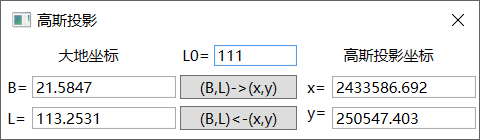
\includegraphics[scale=1]{gaussProj/UI01.png}
    \caption{简单的高斯投影正反算界面}
    \label{fig:GaussProjUI01}
\end{figure}

相应的主要界面代码如下:

\begin{lstlisting}[language=xml]
<TextBlock Text="大地坐标" HorizontalAlignment="Center"
        VerticalAlignment="Center"/>
<TextBlock  Text="B=" Grid.Row="1" Margin="5"/>
<TextBox x:Name="textBox_B" Grid.Row="1"
        Text=""
        VerticalAlignment="Center"  Margin="25,0,0,0"/>
<TextBlock  Text="L=" Margin="5" Grid.Row="2" />
<TextBox x:Name="textBox_L"
        Text=""
        VerticalAlignment="Center" Margin="25,0,0,0" Grid.Row="2" />

<TextBlock  Text="L0=" Grid.Column="1"
        Margin="5,0,0,0" VerticalAlignment="Center"/>
<TextBox x:Name="textBox_L0"
        Text=""
        Grid.Column="1"
        Margin="30,0,3,0" VerticalAlignment="Center"/>
<Button Content="(B,L)->(x,y)" Grid.Column="1" Grid.Row="1"
                Click="BLtoXYButton_Click" Margin="3,3"/>
<Button Content="(B,L)&lt;-(x,y)" Grid.Column="1" Grid.Row="2"
                Click="XYtoBLButton_Click"  Margin="3,3"/>
        
<TextBlock Text="高斯投影坐标" Grid.Column="2"
                HorizontalAlignment="Center" VerticalAlignment="Center"/>
<TextBlock  Text="x=" Margin="5" Grid.Row="1" Grid.Column="2"/>
<TextBox x:Name="textBox_x" Grid.Row="1" Grid.Column="2"
                Text=""
                Margin="25,0,0,0" VerticalAlignment="Center" />
<TextBlock Text="y=" Grid.Row="2" Grid.Column="2" Margin="5,0,0,0"/>
<TextBox x:Name="textBox_y"
                Text=""
                Grid.Row="2"  Grid.Column="2"
                Margin="25,0,0,0" VerticalAlignment="Center" />       
\end{lstlisting}

请注意,在这段xaml界面代码中,由于我们的算法需要与界面上的TextBox控件进行数据交换,
每个TextBox都需要命名(如上的每个TextBox控件都有一个 x:Name 属性)。

相应的正算与反算按钮响应事件代码如下:

\begin{lstlisting}[language=C]
private void BLtoXYButton_Click(object sender, RoutedEventArgs e)
{
    double B, L, L0, x, y;
    double.TryParse(this.textBox_B.Text, out B);
    double.TryParse(this.textBox_L.Text, out L);
    double.TryParse(this.textBox_L0.Text, out L0);

    Spheroid proj = Spheroid.CreateBeiJing1954();
    proj.BLtoXY(
        ZXY.SMath.DMS2RAD(B),
        ZXY.SMath.DMS2RAD(L),
        ZXY.SMath.DMS2RAD(L0),
        out x, out y);
    this.textBox_x.Text = x.ToString();
    this.textBox_y.Text = y.ToString();
}

private void XYtoBLButton_Click(object sender, RoutedEventArgs e)
{
    double B, L, L0, x, y;
    double.TryParse(this.textBox_x.Text, out x);
    double.TryParse(this.textBox_y.Text, out y);
    double.TryParse(this.textBox_L0.Text, out L0);

    Spheroid proj = Spheroid.CreateBeiJing1954();
    proj.XYtoBL(x, y,
        ZXY.SMath.DMS2RAD(L0),
        out B, out L);
    this.textBox_B.Text =ZXY.SMath.RAD2DMS(B).ToString();
    this.textBox_L.Text = ZXY.SMath.RAD2DMS(L).ToString();
}
\end{lstlisting}

在这个两个响应事件中,首先需要直接从界面上的TextBox控件中取值,
由于TextBox的Text属性是文本(string类型),需要用double.TryParse
函数将其转换为double类型。

其次我们默认参考椭球为1954北京坐标系的参考椭球,需要将其创建,此处我们用
类的静态函数可以方便创建,不必记忆其椭球的几何参数值。

然后我们就可以调用我们前边写的正算与反算函数进行高斯投影正反算了,算完后
将值再赋值给相应的TextBox控件的Text属性就可以了。注意传入函数的值如果是度分秒形式的角度,
应该先调用我们前边的写的函数将其转换为弧度,如果算出的值也是角度,也应该调用我们
前面所写的函数将其转换为度分秒形式。


\subsection{界面程序的优化}
上面的简单界面程序存在着一个很大的问题,就是从界面取数据时无法判断数据的有效性等,
也无法发挥WPF界面技术。WPF界面技术里的数据绑定功能(binding)可以很好的简化这一过程。

我们仔细分析前边的界面,这个程序的实质就是一个点的两种形式的坐标之间的转换,
因此我们可以定义一个点类GeoPoint,其定义如下:

\begin{lstlisting}[language=C]
public class GeoPoint
{
    public string Name { get; set;} //点名
    public double B { get; set;}    //纬度,单位:度分秒
    public double L { get; set;}    //经度,单位:度分秒
    public double L0 { get; set;}   //中央子午线经度,单位:度分秒
    public double X { get; set;}    //X坐标
    public double Y { get; set;}    //Y坐标
}
\end{lstlisting}

则在界面代码中可对TextBox的Text做如下绑定:

\begin{lstlisting}[language=C]
<TextBlock Text="大地坐标" HorizontalAlignment="Center"
        VerticalAlignment="Center"/>
<TextBlock  Text="B=" Grid.Row="1" Margin="5"/>
<TextBox x:Name="textBox_B" Grid.Row="1"
        Text="{Binding B, StringFormat={}{0:##0.####}}"
        VerticalAlignment="Center"  Margin="25,0,0,0"/>
<TextBlock  Text="L=" Margin="5" Grid.Row="2" />
<TextBox x:Name="textBox_L"
        Text="{Binding L, StringFormat={}{0:##0.####}}"
        VerticalAlignment="Center" Margin="25,0,0,0" Grid.Row="2" />

<TextBlock  Text="L0=" Grid.Column="1"
        Margin="5,0,0,0" VerticalAlignment="Center"/>
<TextBox x:Name="textBox_L0"
        Text="{Binding L0, StringFormat={}{0:##0.####}}" 
        Grid.Column="1"
        Margin="30,0,3,0" VerticalAlignment="Center"/>
<Button Content="(B,L)->(x,y)" Grid.Column="1" Grid.Row="1"
        Click="BLtoXYButton_Click" Margin="3,3"/>
<Button Content="(B,L)&lt;-(x,y)" Grid.Column="1" Grid.Row="2"
        Click="XYtoBLButton_Click"  Margin="3,3"/>
        
<TextBlock Text="高斯投影坐标" Grid.Column="2"
        HorizontalAlignment="Center" VerticalAlignment="Center"/>
<TextBlock  Text="x=" Margin="5" Grid.Row="1" Grid.Column="2"/>
<TextBox x:Name="textBox_x" Grid.Row="1" Grid.Column="2"
        Text="{Binding X, StringFormat={}{0:##0.###} }"
        Margin="25,0,0,0" VerticalAlignment="Center" />
<TextBlock Text="y=" Grid.Row="2" Grid.Column="2" Margin="5,0,0,0"/>
<TextBox x:Name="textBox_y"
        Text="{Binding Y , StringFormat={}{0:##0.###}}"
        Grid.Row="2"  Grid.Column="2"
        Margin="25,0,0,0" VerticalAlignment="Center" />  
\end{lstlisting}

以上代码中的TextBox控件中的x:Name属性甚至都可以省略。由于这些控件都是
以这个窗体(Window)作为容器的,他们的数据源都可用这个窗体的DataContext
一次性设置,让系统以冒泡的形式自动为属性绑定寻找数据源。窗体为之
设定数据源的代码如下:

\begin{lstlisting}[language=C]
public partial class MainWindow : Window
{
    private GeoPoint geoPoint;
    private Spheroid proj = Spheroid.CreateBeiJing1954();

    public MainWindow()
    {
        InitializeComponent();
        geoPoint = new GeoPoint(){ B= 21.58470845, L= 113.25314880 };
        this.DataContext = geoPoint;
    }
    //.......省略了其他代码......
}
\end{lstlisting}

程序中由于正反算都是基于相同的椭球基准,所以在类MainWindow中定义了
geoPoint实例字段与proj实例字段。在构造函数中为其赋了初值以简化每次在
界面输入数据,为这个窗体的DataContext指定点的各项属性绑定的数据源。

相应的正反算按钮的响应事件修改为:

\begin{lstlisting}[language=C]
private void BLtoXYButton_Click(object sender, RoutedEventArgs e)
{
    double x, y;
    proj.BLtoXY(
        ZXY.SMath.DMS2RAD(geoPoint.B),
        ZXY.SMath.DMS2RAD(geoPoint.L),
        ZXY.SMath.DMS2RAD(geoPoint.L0),
        out x, out y);
    geoPoint.X = x; geoPoint.Y = y;
}

private void XYtoBLButton_Click(object sender, RoutedEventArgs e)
{
    double B, L;
    proj.XYtoBL(geoPoint.X, geoPoint.Y,
       ZXY.SMath.DMS2RAD(geoPoint.L0),
       out B, out L);
    geoPoint.B = ZXY.SMath.RAD2DMS(B);
    geoPoint.L = ZXY.SMath.RAD2DMS(L);
}
\end{lstlisting}

从响应事件可以看出,代码简洁了很多。运行程序时,TextBox框中都有默认数值,
而且非数值数据也输入不进去了,也不需要将文本框中的Text属性转换为double类型了。
一切看似都好,但你发现在点击正算或反算按钮时,界面上的数据没有变化,好像功能没有实现一样,
问题出现在什么地方呢?

我们回过头再看GeoPoint的定义,发现其属性定义过于简单。根据WPF知识可知,在对象属性发生改变时
(如我们的计算中正算改变了X与Y,反算改变了B与L),还需要一种机制通知系统需要刷新界面,
这就需要类GeoPoint从接口 INotifyPropertyChanged 继承并实现它
(该接口所在的命名空间为System.ComponentModel)。修改后的GeoPoint类如下:

\begin{lstlisting}[language=C]
public class GeoPoint : INotifyPropertyChanged
{
    public event PropertyChangedEventHandler PropertyChanged;

    public void RaisePropertyChange(string propertyName)
    {
        if (this.PropertyChanged != null)
        {
            this.PropertyChanged.Invoke(this, 
                new PropertyChangedEventArgs(propertyName));
        }
    }

    private string _name;
    public string Name //点名
    {
        get { return _name; }
        set
        {
            _name = value;
            RaisePropertyChange("Name");
        }
    }

    private double _B;
    public double B //纬度,单位:度分秒
    {
        get { return _B; }
        set
        {
            _B = value;
            RaisePropertyChange("B");
        }
    }

    private double _L;
    public double L //经度,单位:度分秒
    {
        get { return _L; }
        set
        {
            _L = value;
            RaisePropertyChange("L");
        }
    }

    private double _L0;
    public double L0 //中央子午线经度,单位:度分秒
    {
        get { return _L0; }
        set
        {
            _L0 = value;
            RaisePropertyChange("L0");
        }
    }

    private double _X;
    public double X //X坐标
    {
        get { return _X; }
        set
        {
            _X = value;
            RaisePropertyChange("X");
        }
    }
  
    private double _Y;
    public double Y  //Y坐标
    {
        get { return _Y; }
        set
        {
            _Y = value;
            RaisePropertyChange("Y");
        }
    }
}
\end{lstlisting}

与前面的GeoPoint类相比较,现在的这个类从 INotifyPropertyChanged 继承
并实现了接口成员PropertyChanged,在属性值发生改变时利用该接口成员通知界面
属性值发生了变化。

运行程序,功能一切正常。


\subsection{点类的进一步优化}

我们再次审阅界面程序后的正反算代码,发现事实上的正反算都是基于点类的,
也就是说只与GeoPoint类相关,因此我们将正反算功能移到GeoPoint类中,
以进一步简化界面的方法调用。其代码如下:

\begin{lstlisting}[language=C]
public class GeoPoint : INotifyPropertyChanged
{
    //......其它代码.......
    public void BLtoXY(Spheroid spheroid)
    {
        double x, y;
        spheroid.BLtoXY(
           ZXY.SMath.DMS2RAD(this.B),
           ZXY.SMath.DMS2RAD(this.L),
           ZXY.SMath.DMS2RAD(this.L0),
           out x, out y);
        this.X = x; this.Y = y;
    }

    public void XYtoBL(Spheroid spheroid)
    {
        double B, L;
        spheroid.XYtoBL(X, Y, ZXY.SMath.DMS2RAD(this.L0),
           out B, out L);
        this.B = ZXY.SMath.RAD2DMS(B);
        this.L = ZXY.SMath.RAD2DMS(L);
    }
}
\end{lstlisting}

界面正反算代码可以进一步简化为如下形式:

\begin{lstlisting}[language=C]
private void BLtoXYButton_Click(object sender, RoutedEventArgs e)
{
    geoPoint.BLtoXY(proj);
}

private void XYtoBLButton_Click(object sender, RoutedEventArgs e)
{
    geoPoint.XYtoBL(proj) ;
}
\end{lstlisting}

至此,我们的算法与界面几乎是完全分离了,这符合我们第一章所讲的界面与算法相
分离的原则,也为我们的算法进行单元测试和进一步优化迭代打下了基础。


\section{更加实用的多点计算图形程序}

上面的程序从编程的角度讲比较完美了,但从实用的角度来说还有很多缺点,
比如不能选择椭球基准,不能进行多点的正反算,不能读取和写出文本文件数据。
这一节我们将从算法和界面两个方面来构造这个更加实用的多点高斯投影计算的
图形程序。

\subsection{程序的功能}

实用的高斯投影程序功能如下:

\begin{enumerate}
\item 椭球基准的选择:能够自由的选择参考椭球基准,或者自定义参考椭球;
\item 能实现高斯投影正反算与换带功能;
\item 高斯投影坐标的定义:能自动去除或添加点的Y坐标前的常数500km和带号;
\item 数据的界面录入:能利用程序界面组织输入数据;
\item 能导入导出文本数据:能将外部文本数据导入到程序中,能将程序中的数据导出为文本文件;
\item 能实现多个点的批量计算。
\end{enumerate}

软件运行时的界面如图\ref{fig:GaussProjUI02}所示,该界面基本能满足以上功能。

\begin{figure}[htbp]
    \centering
    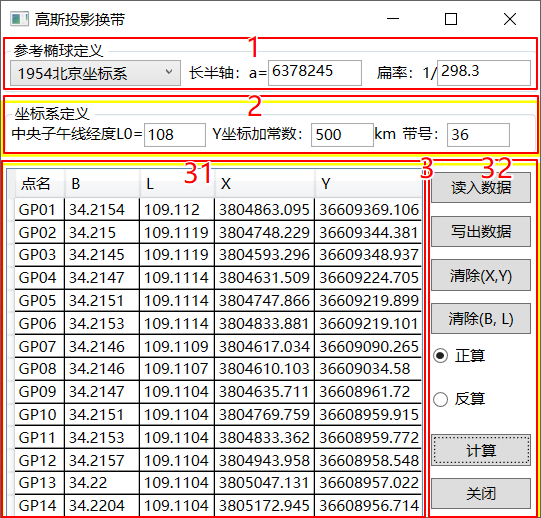
\includegraphics[scale=1]{gaussProj/UI02.png}
    \caption{实用高斯投影程序界面}
    \label{fig:GaussProjUI02}
\end{figure}

\subsection{程序的面向对象分析与实现}

从界面上我们可以看出,程序中应该包含三部分内容:
椭球基准、坐标系、点集。为了满足以上功能,我们需要对我们的程序进行重构。

分析我们前边的 GeoPoint 类会发现,一个点有中央子午线经度 L0 这个属性会很奇怪,
而在实际应用中点集也是基于坐标系的点集,一个点集的y坐标甚至x坐标前的加常数也是基本相同。
因此坐标系应该有中央子午线经度 L0属性,带号N与Y坐标前的加常数YKM,
由于坐标系是依赖于椭球基准的,也应有椭球基准属性ProjSpheroid。
坐标系类的定义如下代码所示:

\begin{lstlisting}[language=C]
using System.Collections.ObjectModel;

/// <summary>
/// 坐标系
/// </summary>
public class CoordinateSystem : INotifyPropertyChanged
{
    //....省略与接口INotifyPropertyChanged有关的代码....

    /// <summary>
    /// 中央子午线经度
    /// </summary>
    private double _L0;
    
    /// <summary>
    /// 中央子午线经度
    /// </summary>
    public double L0
    {
        get { return _L0; }
        set
        {
            _L0 = value;
            RaisePropertyChange("L0");
        }
    }
    
    /// <summary>
    /// 带号
    /// </summary>
    private int _N;
    
    /// <summary>
    /// 带号
    /// </summary>
    public int N
    {
        get { return _N; }
        set
        {
            _N = value;
            RaisePropertyChange("N");
        }
    }
    
    /// <summary>
    /// Y坐标的加常数
    /// </summary>
    private double _YKM;
    
    /// <summary>
    /// Y坐标的加常数
    /// </summary>
    public double YKM
    {
        get { return _YKM; }
        set
        {
            _YKM = value;
            RaisePropertyChange("YKM");
        }
    }
    
    /// <summary>
    /// 坐标点集
    /// </summary>
    private ObservableCollection<GeoPoint>geoPointList = 
        new ObservableCollection<GeoPoint>();
    
    /// <summary>
    /// 坐标点集
    /// </summary>
    public ObservableCollection<GeoPoint> GeoPointList
    {
        get { return geoPointList; }
    }
    
    /// <summary>
    /// 投影椭球基准
    /// </summary>
    private Spheroid spheroid = Spheroid.CreateBeiJing1954();
    
    /// <summary>
    /// 投影椭球基准
    /// </summary>
    public Spheroid ProjSpheroid
    {
        get { return spheroid; }
        set
        {
            spheroid = value;
            RaisePropertyChange("ProjSpheroid");
        }
    }

   public CoordinateSystem(){ }
}
\end{lstlisting}

在类GeoPoint中将属性L0的定义删除。在CoordinateSystem类中,由于
N,L0,YKM需与界面交互,故须从接口 INotifyPropertyChanged 继承。

为了与WPF界面中的DataGrid控件交互,点集需要用 
ObservableCollection<GeoPoint> 表达,不能用List<GeoPoint>,而且默认状态
下就应该生成其实例对象。注意二者的命名空间也不一样,
前者为System.Collections.ObjectModel,
用于界面交互较多,后者为 System.Collections.Generic,用于不需要界面的
算法较多。

为了与界面的初始状态一致,对投影的参考椭球我们默认生成北京54坐标系的
参考椭球。

在我们的程序中GeoPoint类与CoordinateSystem类为了处理与界面交互的
问题,都需要实现接口 INotifyPropertyChanged,实现接口的代码重复。
本着相同或相似的代码在程序中只写一次的原则,我们将这部分的代码独立到
类 NotificationObject 中,让GeoPoint类与CoordinateSystem类从
NotificationObject 类继承。相应的实现代码如下:

\begin{lstlisting}[language=C]
using System.ComponentModel;

namespace GaussProj
{
    public class NotificationObject : INotifyPropertyChanged
    {
        public event PropertyChangedEventHandler PropertyChanged;

        public void RaisePropertyChange(string propertyName)
        {
            if (this.PropertyChanged != null)
            {
                this.PropertyChanged.Invoke(this, new PropertyChangedEventArgs(propertyName));
            }
        }
    }
}

public class GeoPoint : NotificationObject
{
    //删除与NotificationObject类中相同的代码
    //省略GeoPoint类中的内容
}

public class CoordinateSystem : NotificationObject
{
    //删除与NotificationObject类中相同的代码
    //省略CoordinateSystem类中的内容
}
\end{lstlisting}

\subsection{多点的高斯投影计算}

如此,在类CoordinateSystem中就有了用于高斯投影的椭球基准,
有了坐标系的中央子午线经度,有了带号及y坐标前的加常数与点集,
多点的高斯投影计算就万事俱备,只欠实现了。其实现代码如下:

\begin{lstlisting}[language=C]
public class CoordinateSystem : NotificationObject 
{
    //省略其他代码

    /// <summary>
    /// 多点高斯投影正算
    /// </summary>
    public void BLtoXY()
    {
        foreach (var pnt in this.geoPointList)
        {
            pnt.BLtoXY(spheroid, this);
        }
    }

    /// <summary>
    /// 多点高斯投影反算
    /// </summary>
    public void XYtoBL()
    {
        foreach (var pnt in this.geoPointList)
        {
            pnt.XYtoBL(spheroid, this);
        }
    }
}
\end{lstlisting}

从代码中可以看出,在类CoordinateSystem中并没有真正的进行高斯投影正算与
反算,而是通过循环将其委托给每个点的实例了。

点类GeoPoint中的高斯投影正反算实现如下:

\begin{lstlisting}[language=C]
public class GeoPoint : NotificationObject
{
    //省略其他代码
    /// <summary>
    /// 高斯投影正算
    /// </summary>
    /// <param name="spheroid">投影椭球</param>
    /// <param name="cs">坐标系</param>
    public void BLtoXY(Spheroid spheroid, CoordinateSystem cs)
    {
        double x, y;
        spheroid.BLtoXY(
           ZXY.SMath.DMS2RAD(this.B),
           ZXY.SMath.DMS2RAD(this.L),
           ZXY.SMath.DMS2RAD(cs.L0),
           out x, out y);
        this.X = x; this.Y = y + cs.YKM * 1000 + cs.N * 1000000;
    }
    /// <summary>
    /// 高斯投影反算
    /// </summary>
    /// <param name="spheroid">投影椭球</param>
    /// <param name="cs">坐标系</param>
    public void XYtoBL(Spheroid spheroid, CoordinateSystem cs)
    {
        double tB, tL;
        double y = Y - cs.YKM * 1000 - cs.N * 1000000;
        spheroid.XYtoBL(X, y, ZXY.SMath.DMS2RAD(cs.L0),
           out tB, out tL);
        this.B = ZXY.SMath.RAD2DMS(tB);
        this.L = ZXY.SMath.RAD2DMS(tL);
    }
}
\end{lstlisting}

从如上的代码中可以看出,真正的高斯投影正反算还是在我们前面写的Spheroid类中。
请注意在Spheroid类中,所有的与角度有关的单位是弧度,y坐标也是点的真实坐标,
在此我们需要根据坐标系中的信息对其做相应的预处理。

还应注意,在BLtoXY中,为了与界面交互,要赋值给this.X与this.Y,而不是赋值给其变量
this.\_X与this.\_Y。在 XYtoBL 中也同样如此,当然还需要将计算出的弧度值转换为度分秒形式。

\subsection{点坐标数据的读入与写出}

利用我们的界面可以手工输入点的坐标数据,但导入与导出文本数据对于一个
程序来讲是必不可少的功能。

为了避免我们的教学程序过于复杂,我们对数据文件的格式进行适当简化。

在高斯投影正算时,所需的数据应该是:点名,纬度B, 经度L,设计我们的文本文件
内容如下:

\begin{verbatim}
 #点名,   B,   L
GP01,34.2154,109.112
GP02,34.215,109.1119
GP03,34.2145,109.1119
GP04,34.2147,109.1114
GP05,34.2151,109.1114
\end{verbatim}

文件中的每一行第一个字符以 \#开头的我们视为注释行,予以忽略。

在高斯投影反算时,所需的数据应该是:点名,X, Y,设计我们的文本文件
内容如下:

\begin{verbatim}
#点名,       X,       Y,         H
GP01, 3805709.2106, 19333388.3123, 466.419
GP02, 3805595.1034, 19333360.1973, 470.94
GP03, 3805440.0738, 19333360.1727, 478.728
GP04, 3805481.9494, 19333237.0999, 475.975
GP05, 3805598.4201, 19333235.7343, 469.738
\end{verbatim}

文件中的数据项可以多余三项,我们只读取第1、2、3项,其余忽略。

在写出数据时,我们将点的五项数据:点名,B, L, X, Y 全部写出,
如下所示:

\begin{verbatim}
# 点名,    B,      L,     X,      Y 
GP01, 34.2154, 109.112  , 3804863.095, 36609369.106
GP02, 34.215,   109.1119, 3804748.229, 36609344.381
GP03, 34.2145, 109.1119, 3804593.296, 36609348.937
GP04, 34.2147, 109.1114, 3804631.509, 36609224.705
GP05, 34.2151, 109.1114, 3804747.866, 36609219.899
\end{verbatim}

用户在使用时可以将其数据拷贝到Word中按分隔符 ``,''生成表格进行编辑
处理,或按分隔符 ``,''导入到Excel中进行编辑排版处理。

读入的点坐标数据应存储在我们的程序中,很显然应该在类CoordinateSystem中
实现读入文本文件数据功能,写出数据的功能也如此,其实现代码如下:

\begin{lstlisting}[language=C]
public class CoordinateSystem : NotificationObject 
{
    //省略其他代码

    /// <summary>
    /// 读入点集坐标数据
    /// </summary>
    /// <param name="fileName">文件名</param>
    /// <param name="format">点的坐标格式:BL-Name,B,L  
    ///                                 XY-Name,X,Y
    /// </param>
    public void ReadGeoPointData(string fileName, string format)
    {
        using (System.IO.StreamReader sr = new System.IO.StreamReader(fileName) )
        {
            string buffer;
            //读入点的坐标数据
            this.GeoPointList.Clear();
            while (true)
            {
                buffer = sr.ReadLine();
                if (string.IsNullOrEmpty(buffer)) break; //文件末尾或空行退出
                if (buffer[0] == '#') continue;
                string[] its = buffer.Split(new char[1] { ',' });
                if (its.Length < 3) continue; //少于三项数据,不是点的坐标数据,忽略
                GeoPoint pnt = new GeoPoint();
                pnt.Name = its[0].Trim(); 
                if (format == "XY")
                {                       
                    pnt.X = double.Parse(its[1]); 
                    pnt.Y = double.Parse(its[2]);
                    pnt.B = 0; pnt.L = 0;
                }
                else if (format == "BL")
                {
                    pnt.B = double.Parse(its[1]); 
                    pnt.L = double.Parse(its[2]); 
                    pnt.X = 0; pnt.Y = 0;
                }
               
                this.GeoPointList.Add(pnt);
            }
        }
    }

    /// <summary>
    /// 写出点集坐标数据
    /// </summary>
    /// <param name="fileName">文件名</param>
    public void WriteGeoPointData(string fileName)
    {
        using (System.IO.StreamWriter sr = new System.IO.StreamWriter(fileName))
        {
            sr.WriteLine("#点名,   B,   L,  X,  Y");
            foreach (var pnt in this.geoPointList)
            {
                sr.WriteLine( pnt );
            }
        }
    }
}
\end{lstlisting}

写数据比较简单,按要求写出即可,需要注意的是第57行,在函数WriteLine中
我们直接写出了GeoPoint的实例对象pnt,这需要在GeoPoint中将ToString()
进行override,实现代码如下:
\begin{lstlisting}[language=C]
public class GeoPoint : NotificationObject
{
    public override string ToString()
    {
        return string.Format("{0},{1:0.0000},{2:0.0000},{3:0.000},{4:0.000}", Name, B, L, X, Y);
    }
}
\end{lstlisting}

在占位符中我们加入了输出浮点数据的格式控制,保证输出的角度小数位数不超过四位,
输出的坐标不超过三位。

读入数据相对于写出数据要由于需要解码数据,所以要复杂一些。小于三个数据项
的行我们直接略过,同时我们能加入格式控制,如果格式控制BL,
意味着数据文件是经纬度数据,其他属性相应置零。

读入数据的这段代码我们实现的方式较为粗略,只是通过逗号分隔的数据项个数
进行了判断,这在真正的程序开发中是不可靠的,可以通过正则表达式对每行数据进行检验,
对符合要求的文本数据加以处理,以此来提高读取文本数据功能的容错能力。

清除(X, Y)与清除(B, L)功能实质上是将点的这些属性置零,比较简单,相应代码如下:

\begin{lstlisting}[language=C]
public class CoordinateSystem : NotificationObject 
{
    //省略其他代码

    public void ClearXY()
    {
        foreach (var pnt in this.geoPointList)
        {
            pnt.X = pnt.Y = 0;
        }
    }
    public void ClearBL()
    {
        foreach (var pnt in this.geoPointList)
        {
            pnt.B = pnt.L = 0;
        }
    }
}
\end{lstlisting}


\subsection{界面设计与实现}

按图\ref{fig:GaussProjUI02}设计的界面代码如下:

\begin{lstlisting}[language=xml]
<Window x:Class="GaussProj.GaussProjWin"
        xmlns="http://schemas.microsoft.com/winfx/2006/xaml/presentation"
        xmlns:x="http://schemas.microsoft.com/winfx/2006/xaml"
        xmlns:d="http://schemas.microsoft.com/expression/blend/2008"
        xmlns:mc="http://schemas.openxmlformats.org/markup-compatibility/2006"
        xmlns:local="clr-namespace:GaussProj"
        mc:Ignorable="d"
        Title="高斯投影换带" Height="360" Width="540">
    <Grid>
        <Grid.RowDefinitions>
            <RowDefinition Height="45"/>
            <RowDefinition Height="5"/>
            <RowDefinition Height="45"/>
            <RowDefinition Height="5"/>
            <RowDefinition Height="Auto"/>
        </Grid.RowDefinitions>
        <GroupBox x:Name="groupBox_spheroid" Header="参考椭球定义" 
            DataContext="ProjSpheroid" Margin="1">
            <Grid>
                <Grid.ColumnDefinitions>
                    <ColumnDefinition Width="200*"/>
                    <ColumnDefinition Width="70"/>
                    <ColumnDefinition Width="110*"/>
                    <ColumnDefinition Width="60"/>
                    <ColumnDefinition Width="110*"/>
                </Grid.ColumnDefinitions>
                <ComboBox Grid.Column="0" x:Name="comboBox_Spheroid" 
                          SelectionChanged="comboBox_Spheroid_SelectionChanged">
                    <ComboBoxItem  Content="1954北京坐标系" Tag="BJ1954"/>
                    <ComboBoxItem Content="1980西安坐标系" Tag="XA1980"/>
                    <ComboBoxItem Content="CGCS2000大地坐标系" Tag="CGCS2000"/>
                    <ComboBoxItem Content="自定义参考椭球" Tag="CS0000"/>
                </ComboBox>
                <TextBlock Text="长半轴:a=" Grid.Column="1" 
                    VerticalAlignment="Center" HorizontalAlignment="Right"/>
                <TextBox x:Name="textBox_a" Grid.Column="2" Text="{Binding a}"/>
                <TextBlock Text="扁率:1/" Grid.Column="3" 
                    VerticalAlignment="Center" HorizontalAlignment="Right"/>
                <TextBox x:Name="textBox_f" Grid.Column="4" Text="{Binding f}"/>
            </Grid>
        </GroupBox>

        <Border  Grid.Row="2" BorderBrush="Yellow" BorderThickness="2">
            <GroupBox x:Name="groupBox_CoordinateSystem" Header="坐标系定义">
            <StackPanel Orientation="Horizontal">
                <TextBlock Text="中央子午线经度L0=" />
                <TextBox x:Name="textBox_L0" Text="{Binding L0}" Width="50"/>
                <TextBlock Text="Y坐标加常数:" Margin="5,0,0,0" />
                <TextBox x:Name="textBox_YKM" Text="{Binding YKM}" Width="50"/>
                <TextBlock Text="km" />
                <TextBlock Text="带号:" Margin="5,0,0,0"/>
                <TextBox x:Name="textBox_N" Text="{Binding N}" Width="50"/>
            </StackPanel>
            </GroupBox>
        </Border>
        
        <Border  Grid.Row="4" BorderBrush="Yellow" BorderThickness="2">
            <Grid>
                <Grid.ColumnDefinitions>
                    <ColumnDefinition Width="200*"/>
                    <ColumnDefinition Width="90"/>
                </Grid.ColumnDefinitions>
                <DataGrid x:Name="dataGrid_ctrPnt" 
                    AutoGenerateColumns="False" Margin="2" 
                    ItemsSource="{Binding GeoPointList}" >
                <DataGrid.Columns>
                    <DataGridTextColumn Header="点名" 
                        Binding="{Binding Name}"
                        MinWidth="40"/>
                    <DataGridTextColumn Header="B" 
                        Binding="{Binding B , StringFormat={}{0:##0.####}}" 
                        MinWidth="60"/>
                    <DataGridTextColumn Header="L" 
                        Binding="{Binding L , StringFormat={}{0:##0.####}}" 
                        MinWidth="60"/>
                    <DataGridTextColumn Header="X" 
                        Binding="{Binding X , StringFormat={}{0:##0.###}}" 
                        MinWidth="60"/>
                    <DataGridTextColumn Header="Y" 
                        Binding="{Binding Y, StringFormat={}{0:##0.###}}"
                        MinWidth="60" />
                </DataGrid.Columns>
            </DataGrid>

                <StackPanel Grid.Column="1" Orientation="Vertical">
                    <RadioButton x:Name="radioButton_BLtoXY"  Content="正算" 
                        Height="25" Width="80" Margin="5"/>
                    <RadioButton x:Name="radioButton_XYtoBL"  Content="反算" 
                        IsChecked="True" Height="25" Width="80" Margin="5" />

                    <Button x:Name="Button_ReadGaussProjData" Content="读入数据"
                        Height="25" Width="80" Margin="5" 
                        Click="Button_ReadGaussProjData_Click"/>
                    <Button x:Name="Button_WriteGaussProjData" Content="写出数据" 
                        Height="25" Width="80" Margin="5" 
                        Click="Button_WriteGaussProjData_Click"/>

                    <Button x:Name="Button_ClearXY" Content="清除(X,Y)" 
                        Height="25" Width="80" Margin="5" 
                        Click="Button_ClearXY_Click"/>
                    <Button x:Name="Button_ClearBL" Content="清除(B, L)" 
                        Height="25" Width="80" Margin="5" 
                        Click="Button_ClearBL_Click"/>
                    
                    <Button x:Name="Button_CalGaussProj"  Content="计算" 
                        Height="25" Width="80" Margin="5" 
                        Click="Button_CalGaussProj_Click"/>
                    <Button x:Name="Button_Close" Content="关闭" 
                        Height="25" Width="80" Margin="5" 
                        Click="Button_Close_Click"/>
                </StackPanel>
            </Grid>
        </Border>     
    </Grid>
</Window>
\end{lstlisting}

在这段xaml代码中,除了功能按钮区外,实际上分为了三部分:

第一部分为参考椭球定义,如第18行代码所示,我们将其属性布局到
 groupBox\_spheroid中,数据绑定a与f,数据源设置在groupBox\_spheroid中,
 采用冒泡搜寻类CoordinateSystem中的ProjSpheroid属性。

 ComboBox中的参考椭球类型采用了硬编码方式直接写在其中了。通过SelectionChange
 事件对不同选择进行响应。

第二部分为坐标系定义,同样采用数据绑定的形式与界面交互数据,数据源来自
类CoordinateSystem。

第三部分为点集部分,数据源为类CoordinateSystem中的GeoPointList属性,如
第65行代码所示。

界面后台代码如下:

\begin{lstlisting}[language=C]
public partial class GaussProjWin : Window
{       
    private CoordinateSystem myCoordinateSystem;

    public GaussProjWin()
    {
        InitializeComponent();

        myCoordinateSystem = new CoordinateSystem() {
            L0 = 111, N = 19, YKM = 500};
        this.DataContext = myCoordinateSystem;

        this.comboBox_Spheroid.SelectedIndex = 0;
    }

    //省略其他代码
}
\end{lstlisting}

在窗体后台代码中,我们设置了窗体类的类实例变量myCoordinateSystem完成
各项功能。在其窗体类的构造函数中实例化并对其属性赋了初始值,同时将
窗体的DataContex属性设为myCoordinateSystem,完成数据绑定的数据源设置。
同时为了维持与界面属性的一致性,将comboBox\_Spheroid的SelectedIndex设为0。

界面的其它功能按钮的实现比较简单,实现代码如下:

\begin{lstlisting}[language=C]
public partial class GaussProjWin : Window
{   
    //省略其他代码

    private void comboBox_Spheroid_SelectionChanged(object sender, 
        SelectionChangedEventArgs e)
    {
        if(comboBox_Spheroid.SelectedIndex == 0)
            myCoordinateSystem.ProjSpheroid = Spheroid.CreateBeiJing1954();
        else if (comboBox_Spheroid.SelectedIndex == 1)
            myCoordinateSystem.ProjSpheroid = Spheroid.CreateXian1980();
        else if (comboBox_Spheroid.SelectedIndex == 2)
            myCoordinateSystem.ProjSpheroid = Spheroid.CreateCGCS2000();
        else if (comboBox_Spheroid.SelectedIndex == 3)
            myCoordinateSystem.ProjSpheroid = 
                Spheroid.CreateCoordinateSystem(6378137, 298.257222101);
        this.groupBox_spheroid.DataContext = myCoordinateSystem.ProjSpheroid;
    }

    private void Button_ReadGaussProjData_Click(object sender,
        RoutedEventArgs e)
    {
        OpenFileDialog dlg = new OpenFileDialog();
        dlg.DefaultExt = ".txt";
        dlg.Filter = "高斯投影坐标数据|*.txt|All File(*.*)|*.*";
        if (dlg.ShowDialog() != true) return;

        if (this.radioButton_BLtoXY.IsChecked == true)
            myCoordinateSystem.ReadGeoPointData(dlg.FileName, "BL");
        else if(this.radioButton_XYtoBL.IsChecked == true)
            myCoordinateSystem.ReadGeoPointData(dlg.FileName, "XY");
    }

    private void Button_WriteGaussProjData_Click(object sender, 
        RoutedEventArgs e)
    {
        SaveFileDialog dlg = new SaveFileDialog();
        dlg.DefaultExt = ".txt";
        dlg.Filter = "高斯投影坐标数据|*.txt|All File(*.*)|*.*";
        if (dlg.ShowDialog() != true) return;

        myCoordinateSystem.WriteGeoPointData(dlg.FileName);
    }

    private void Button_ClearXY_Click(object sender, RoutedEventArgs e)
    {
        myCoordinateSystem.ClearXY();
    }

    private void Button_ClearBL_Click(object sender, RoutedEventArgs e)
    {
        myCoordinateSystem.ClearBL();
    }

    private void Button_CalGaussProj_Click(object sender, RoutedEventArgs e)
    {
        if (radioButton_BLtoXY.IsChecked == true)
            myCoordinateSystem.BLtoXY();
        else if (radioButton_XYtoBL.IsChecked == true)
            myCoordinateSystem.XYtoBL();
    }

    private void Button_Close_Click(object sender, RoutedEventArgs e)
    {
        this.Close();
    }
}
\end{lstlisting}

\subsection{换带功能的实现}

在我们以上的设计中好像没有换带计算,虽然没有直接实现,但确实是实现了。
在前边的论述中,我们讲过,换带计算的实质是变换坐标系的中央子午线位置,
过程为:先进行坐标反算,然后变换中央子午线经度,再反算新的坐标即可。

\begin{figure}[htbp]
    \centering
    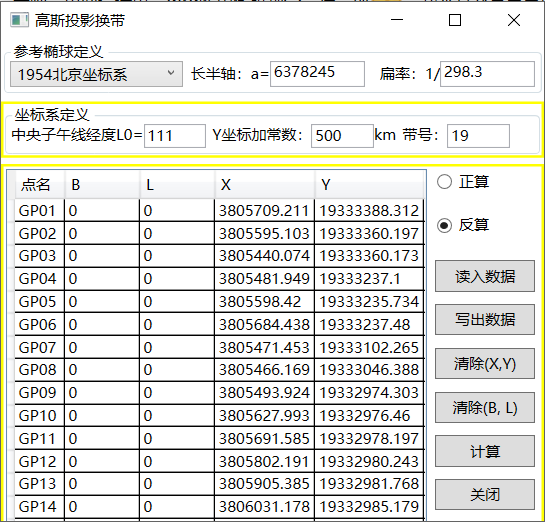
\includegraphics[scale=0.8]{gaussProj/UI03.png}
    \caption{$6\degree$带第19带数据界面}
    \label{fig:GaussProjUI03}
\end{figure}

启动程序,在反算的模式下读入数据,如图\ref{fig:GaussProjUI03}所示,这是一6度带第
19带的北京54坐标:

点击计算,反算各点的大地坐标经纬度,如图\ref{fig:GaussProjUI04}所示。

\begin{figure}[htbp]
    \centering
    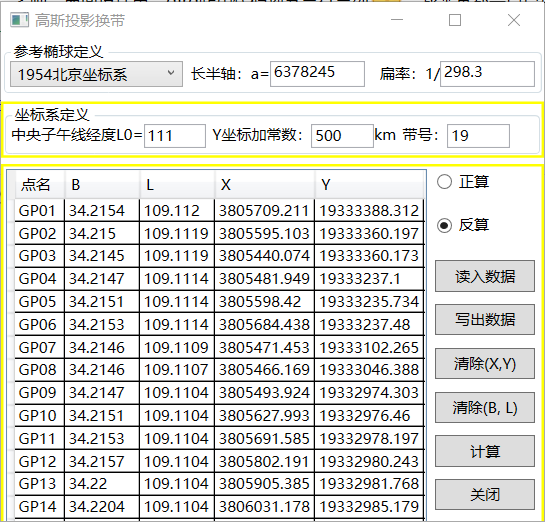
\includegraphics[scale=0.8]{gaussProj/UI04.png}
    \caption{$6\degree$带第19带反算数据界面}
    \label{fig:GaussProjUI04}
\end{figure}

现在我们准备将其换带到3度带的38带坐标系去,设置中央子午线经度L0为108,
带号设为36,选择正算,点击清除(x,y)按钮将X,Y坐标设置为0,如图\ref{fig:GaussProjUI05}所示:

\begin{figure}[htbp]
    \centering
    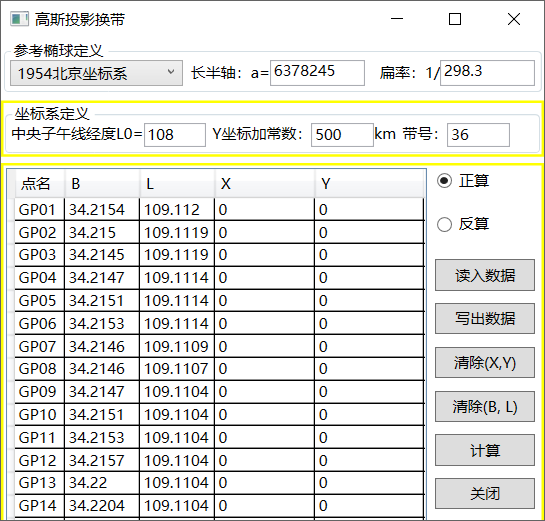
\includegraphics[scale=0.8]{gaussProj/UI05.png}
    \caption{设置$3\degree$带第36带数据界面}
    \label{fig:GaussProjUI05}
\end{figure}

点击计算按钮,计算出新坐标系下各点的坐标,如图\ref{fig:GaussProjUI06}所示:
\begin{figure}[htbp]
    \centering
    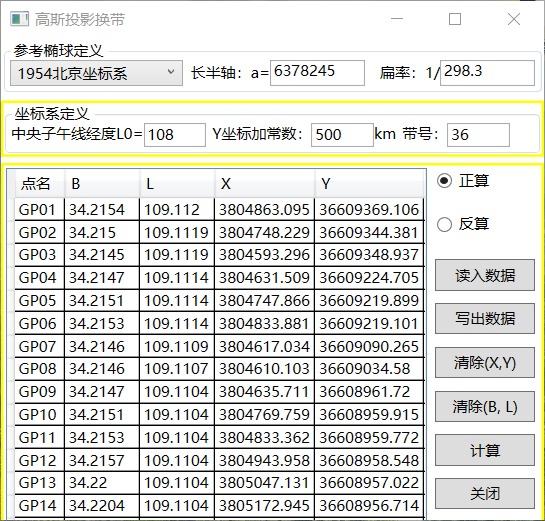
\includegraphics[scale=0.8]{gaussProj/UI06.png}
    \caption{$3\degree$带第36带正算数据界面}
    \label{fig:GaussProjUI06}
\end{figure}

到此就完成了换带功能,可以点击写出数据按钮将计算成果输出。

\subsection{注意事项与功能扩展}

以上过程也可以看成是我们这个软件的教程。但应注意,换带计算只限于相同椭球
基准的情况才能应用,不能在不同椭球基准间应该该功能。

以上换带功能也可以设计一个界面,在新的界面上将新旧坐标系的中央子午线经度
都设置出,从而完成一键式换带计算功能。

我们经常在一些资料中见到椭球膨胀法建立独立坐标系或施工坐标系的方法,
椭球膨胀法是依据某种给定的参考椭球,根据测区的平均高程和平距纬度将
椭球面扩大而维持扁率不变,也可以应用换带的方法将椭球膨胀后的坐标与原坐标系的
坐标进行相互转换。但应注意椭球膨胀后,各个点的纬度值也会发生变化,
在这种换带过程中需要修正各个点的纬度值,大家可以参看这方面的资料。

随着我国现在对CGCS2000大地坐标系的推广应用,大家还可以将大地坐标(B,L)
与空间直角坐标(X,Y,Z)进行相互转换,这样就可以实现空间直角坐标(X,Y,Z)
到高斯平面坐标之间的计算了。进而在桌面端电脑或移动设备上编程实现更多的功能应用。

大地坐标(B,L,H)与空间直角坐标(X,Y,Z)的相互转换公式如下:

已知大地坐标计算空间直角坐标的公式:
\[
\left \{ \begin{aligned}
X &= (N+H) \cos B \cos L \\
Y &= (N+H) \cos B \sin L \\
Z &= [N(1 - e^2) + H)] \sin B 
\end{aligned} \right.
\]

已知空间直角坐标计算大地坐标的公式如下:

\[
\left \{ \begin{aligned}
L &= \arctan \frac{Y}{X} \\
\tan B &= \frac{Z + Ne^2 \sin B}{\sqrt{X^2 + Y^2}} \\
H &= \frac{Z}{sinB} - N(1-e^2) 
\end{aligned} \right.
\]

本处只是列出了计算公式,大家可以查找资料寻找更加高效的计算方法。

\section*{小结}

我们从一个较为简单的单点高斯投影正反算程序开始,运用
C\#知识与WPF界面技术实现了一个较为实用的高斯投影正反算与换带
程序。

在程序过程中,我们遵循了界面与算法相分离的原则,运用了WPF的
事件绑定等技术。

这个程序从功能上讲还是有许多不足的,从易用性上也还有许多值得改进的
地方。希望随着我们的C\#知识与WPF技术的积累,能在以后将它优化得更好!

%%% Local Variables:
%%% mode: latex
%%% TeX-master: "../clcxsj"
%%% End:
                   %%高斯投影程序设计
%!TEX root = ../clcxsj.tex

\chapter{平面坐标系统之间的转换}

在某些工程中,由于不知道新旧两种坐标系的建立方法或参数,因此无法用换带计算的方法
进行坐标转换。如果知道某些点在两个坐标系中的坐标值,我们就可以采用一些近似的转换方
法将其它的点也转换到新坐标系中,求出其坐标值。尤其对于较低等级的大量控制点来说,
采用这些近似方法,能够快速得到转换结果。

 \section{原理和数学模型}

\subsection{原理}
这些方法的实质是根据新旧网的重合点(又称为公共点)的坐标值之差,按一定的规律修正
旧网的各点坐标值,使旧网最恰当的配合到新网内。修正时因不合观测值改正数平方和为最
小的原则,故为近似方法。

\begin{figure}[htbp]
    \centering
    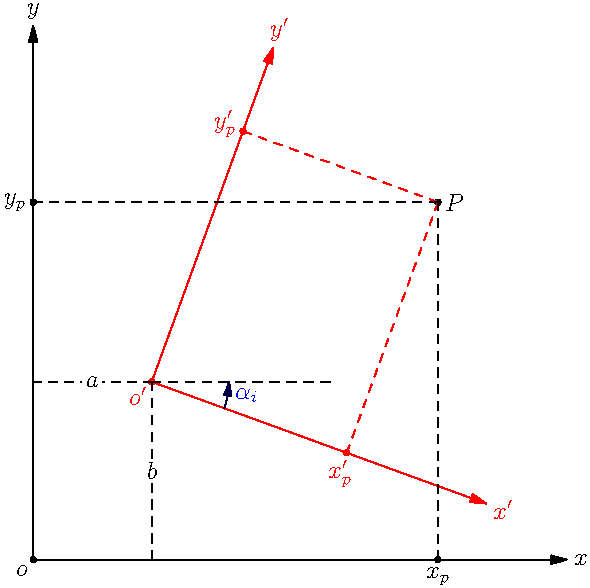
\includegraphics[scale=1]{xytoxy/xytoxy.pdf}
    \caption{坐标相似变换示意图}
    \label{fig:xytoxy}
\end{figure}

常用的方法有简单变换方法(又称赫尔默特法或相似变换法)、仿射变换法、正形变换法等。
在这里我们主要讲解简单变换法。

\subsection{相似变换法的数学模型}
实质是使旧网坐标系平移、旋转和进行尺度因子改正,将旧网配合到新网上。因旧网形状保
持不变,故称为平面相似变换法。

变换方程为:
$$\left.
\begin{array}{l}
\textrm{$x=a+k(x'\cos\alpha+y'\sin\alpha)$} \\
\textrm{$y=b+k(-x'\sin\alpha+y'\cos\alpha)$}
\end{array}\right\}$$

式中$a$,$b$表示平移,$\alpha$是旧网$x'$轴逆转至新网$x$轴的转角,$k$为尺度因子。
这些变换参数是未知的,要根据新旧网公共点上的已知坐标$x$,$y$和$x'$、$y'$求解确定。

因此必须至少有两个公共点,列出四个方程式,解算出这四个未知参数值。如果具有两个以
上的公共点时,就应该应用最小二乘平差方法,求解最或是参数值。

为解算出这些参数,我们引入参数$c$、$d$:

$c=k\cos\alpha$,$d=k\sin\alpha$

将公式转换为:
$$\left.
\begin{array}{l}
\textrm{$x=a+x'c+y'd$}\\
\textrm{$y=b+y'c-x'd¥$}
\end{array}\right\}$$

由于新旧网都存在测量误差,设新旧坐标$x$,$y$和$x'$,$y'$的误差分别为
$v_x$,$v_y$和$v_{x'}$,$v_{y'}$,因此上式改写为:

$$\left.\begin{array}{l}
\textrm{$x+v_x=a+(x'+v_{x'})c+(y'+v_{y'})d$} \\
\textrm{$y+v_y=b+(y'+v_{y'})c-(x'+v_{x'})d$}
\end{array}\right\}$$

设:
$$\left.\begin{array}{l}
\textrm{$n_x=-v_x+cv_{x'}+dv_{y'}$} \\
\textrm{$n_y=-v_y-dv_{x'}+cv_{y'}$}
\end{array}\right\}$$

则有:
$$\left.\begin{array}{l}
\textrm{$-n_x=a+x'c+y'd-x$} \\
\textrm{$-n_y=b+y'c-x'd-y$}
\end{array}\right\}$$

若有$r$个新旧网的公共点,则可组成$r$对方程:
$$V=BX-l$$

上式即为参数平差时的方程,$l$代表观测向量,$V$代表改正数向量,$B$代表系数矩阵,
$X$是参数向量。它们的值为:

$\mathbf{V}=
\left(\begin{array}{c}
-n_{x1} \\ -n_{y1} \\ \vdots \\ -n_{xr} \\ -n_{yr}
\end{array}\right)$
$\mathbf{B}=
\left(\begin{array}{cccc}
1 & 0 & x'_1 & y'_1 \\
0 & 1 & y'_1 & -x'_1 \\
\dots & \dots & \ldots & \ldots \\
1 & 0 & x'_r & y'_r \\
0 & 1 & y'_r & -x'_r
\end{array}\right)$
$\mathbf{X}=
\left(\begin{array}{c}
a \\ b \\ c \\ d
\end{array}\right)$
$\mathbf{l}=
\left(\begin{array}{c}
x_1 \\ y_1 \\ \vdots \\ x_r \\ y_r
\end{array}\right)$

根据最小二乘原理$V^TV=min$可得到法方程:
$$B^TBX-B^Tl=0$$

解法方程可求得$a$、$b$、$c$、$d$的值:
$$X=(B^TB)^{-1}(B^Tl)$$

旋转角$\alpha$和尺度比$k$为:
$$\alpha=\arctan\frac{d}{c}$$
$$k=\sqrt{c^2+d^2}$$
之后,就可计算旧网中所有待转换点的新坐标。

请注意,以上图及公式推导是按数学坐标系进行的,在用测量坐标代入计算时
应将测量坐标$(x,y)$以$(y,x)$形式代入,否则应对以上图形与公式进行变换。

\section{程序设计与实现}

程序整体功能比较单一,从数学模型分析可看出,程序的关
键是在于如何组成系数矩阵$B$与常数项$l$。

\subsection{程序功能分析}

在程序中,我们需要能够有录入数据界面手工输入数据,能够导入与导出
文本文件形式组织的数据,能够输出计算成果,能够计算转换系数或根据已有的
转换系数也能计算待计算点在新坐标系中的坐标。

由此,我们设计出程序界面如图\ref{fig:XYtoXYUI02}所示:

\begin{figure}[htbp]
    \centering
    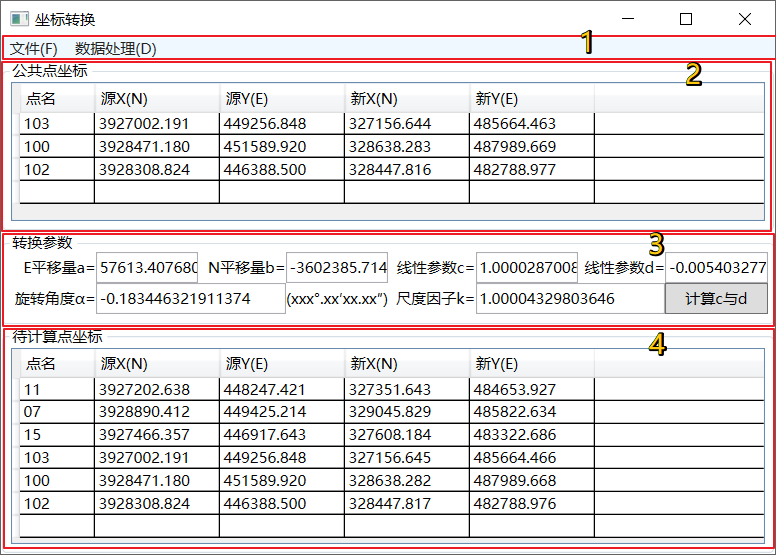
\includegraphics[scale=0.8]{xytoxy/XYtoXYUI02.png}
    \caption{坐标转换程序界面}
    \label{fig:XYtoXYUI02}
\end{figure}

\subsection{程序界面设计}

由图\ref{fig:XYtoXYUI02}分析可知,界面分为菜单、公共点坐标、转换参数与
待计算点坐标四个部分。

整个界面采用DockPanel布局,以加入菜单项,使用菜单项进行功能计算可以有效节省
界面的布局空间。余下的部分采用Grid布局,将其划分为三行,
即三个部分。第一行中加入GroupBox控件作为标题,在其中加入DataGrid控件;
第二部分中加入Grid布局,将其二行八列进行布局;第三部分同第一部分一样。

由于需要根据输入的a、b、$\alpha$、k计算各点在新坐标系中的坐标,为了输入
旋转角度的便捷性(直接输入度分秒),因此加入了计算c与d的按钮。程序中计算各待计算点坐标
时实际使用的参数是$a,b,c,d$。

整个界面布局xaml代码如下:
\begin{lstlisting}[language=xml]
<DockPanel LastChildFill="True">
    <Menu  x:Name="mainmenu" DockPanel.Dock="Top" Background="AliceBlue">
        <MenuItem Header="文件(F)">
            <MenuItem Header="打开文本数据"
               Click="menuItem_OpenTextFileData_Click"/>
            <MenuItem Header="保存文本数据"
                Click="menuItem_SaveTextFileData_Click"/>
            <Separator/>
            <MenuItem Header="退出" Click="menuItem_Exit_Click"/>
       </MenuItem>
        <MenuItem Header="数据处理(D)">
            <MenuItem Header="计算转换参数" 
                Click="menuItem_CalCoefficient_Click" />
            <MenuItem Header="计算待计算点坐标" 
                Click="menuItem_Cal_UnKnw_XY_Click" />
            <Separator/>
            <MenuItem Header="写出计算成果" 
                Click="menuItem_Write_Result_Click" />
        </MenuItem>
    </Menu>

    <Grid>
        <Grid.RowDefinitions>
            <RowDefinition Height="150*"/>
            <RowDefinition Height="75"/>
            <RowDefinition Height="200*"/>
        </Grid.RowDefinitions>
        <GroupBox Header="公共点坐标" Grid.Row="0">
        <DataGrid AutoGenerateColumns="False" Margin="2" 
            ItemsSource="{Binding KnwPointList}">
            <DataGrid.Columns>
                <DataGridTextColumn Header="点名" MinWidth="60"
                    Binding="{Binding Name}"  />
                <DataGridTextColumn Header="源X(N)" MinWidth="100"
                    Binding="{Binding OX, StringFormat={}{0:0.000}}"/>
                <DataGridTextColumn Header="源Y(E)" MinWidth="100"
                    Binding="{Binding OY, StringFormat={}{0:0.000}}"/>
                <DataGridTextColumn Header="新X(N)"  MinWidth="100"
                    Binding="{Binding NX, StringFormat={}{0:0.000}}"/>
                <DataGridTextColumn Header="新Y(E)" MinWidth="100"
                    Binding="{Binding NY, StringFormat={}{0:0.000}}"/>
            </DataGrid.Columns>
        </DataGrid>
            </GroupBox>

            <GroupBox Header="转换参数" Grid.Row="1">
                <Grid>
                    <Grid.ColumnDefinitions>
                        <ColumnDefinition Width="70"/>
                        <ColumnDefinition Width="120*"/>
                        <ColumnDefinition Width="70"/>
                        <ColumnDefinition Width="120*"/>
                        <ColumnDefinition Width="70"/>
                        <ColumnDefinition Width="120*"/>
                        <ColumnDefinition Width="70"/>
                        <ColumnDefinition Width="120*"/>
                    </Grid.ColumnDefinitions>
                    <Grid.RowDefinitions>
                        <RowDefinition Height="25"/>
                        <RowDefinition Height="25"/>
                    </Grid.RowDefinitions>
                    <TextBlock Text="E平移量a=" Grid.Row="0" Grid.Column="0" 
                        VerticalAlignment="Center" HorizontalAlignment="Right"/>
                    <TextBox x:Name="textBox_a" Grid.Row="0" Grid.Column="1" 
                        Text="{Binding a}" 
                        VerticalContentAlignment="Center"/>
                    <TextBlock Text="N平移量b=" Grid.Row="0" Grid.Column="2"  
                        VerticalAlignment="Center" HorizontalAlignment="Right"/>
                    <TextBox x:Name="textBox_b" Grid.Row="0" Grid.Column="3"  
                        Text="{Binding b}"
                        VerticalContentAlignment="Center"/>
                    <TextBlock Text="线性参数c=" Grid.Row="0" Grid.Column="4" 
                        VerticalAlignment="Center" HorizontalAlignment="Right"/>
                    <TextBox x:Name="textBox_c" Grid.Row="0" Grid.Column="5" 
                        Text="{Binding c}"
                        VerticalContentAlignment="Center"/>
                    <TextBlock Text="线性参数d=" Grid.Row="0" Grid.Column="6" 
                        VerticalAlignment="Center" HorizontalAlignment="Right"/>
                    <TextBox x:Name="textBox_d" Grid.Row="0" Grid.Column="7"  
                        Text="{Binding d}" 
                        VerticalContentAlignment="Center"/>
                    <TextBlock Text="旋转角度α=" Grid.Row="1" Grid.Column="0" 
                        VerticalAlignment="Center" HorizontalAlignment="Right"/>
                    <TextBox x:Name="textBox_alpha" Grid.Row="1" Grid.Column="1"  
                        Text="{Binding alpha}" 
                        Grid.ColumnSpan="2"
                        VerticalContentAlignment="Center"/>
                    <TextBlock Text="(xxx°.xx′xx.xx″)" Grid.Row="1" Grid.Column="3" 
                        VerticalAlignment="Center" HorizontalAlignment="Right"/>
                    <TextBlock Text="尺度因子k=" Grid.Row="1" Grid.Column="4" 
                        VerticalAlignment="Center" HorizontalAlignment="Right"/>
                    <TextBox x:Name="textBox_k" Grid.Row="1" Grid.Column="5" 
                        Text="{Binding k}" 
                        Grid.ColumnSpan="2"
                        VerticalContentAlignment="Center"/>
                    <Button x:Name="button_Cal_cd"  Content="计算c与d"
                        Grid.Row="1" Grid.Column="7" 
                        Click="button_Cal_cd_Click"/>
                </Grid>
            </GroupBox>

            <GroupBox Header="待计算点坐标" Grid.Row="2">
                <DataGrid AutoGenerateColumns="False" Margin="2" 
                    ItemsSource="{Binding UnKnwPointList}">
                    <DataGrid.Columns>
                        <DataGridTextColumn Header="点名" MinWidth="60"
                            Binding="{Binding Name}"  />
                        <DataGridTextColumn Header="源X(N)"  MinWidth="100"
                            Binding="{Binding OX, StringFormat={}{0:0.000}}"/>
                        <DataGridTextColumn Header="源Y(E)" MinWidth="100"
                            Binding="{Binding OY, StringFormat={}{0:0.000}}"/>
                        <DataGridTextColumn Header="新X(N)" MinWidth="100"
                            Binding="{Binding NX,StringFormat={}{0:0.000}}" />
                        <DataGridTextColumn Header="新Y(E)" MinWidth="100"
                            Binding="{Binding NY, StringFormat={}{0:0.000}}" />
                    </DataGrid.Columns>
                </DataGrid>
            </GroupBox>
        </Grid>
    </DockPanel>
\end{lstlisting}

\subsection{数据文件和成果文件格式}
由于程序的功能较为单一,数据文件的格式也较为简单。我们设计格式如下:
\begin{verbatim}
#赫尔默特四参数转换法数据文件
#每行以“#”开头的行均被认为是注释行
#公共点在源坐标系中的坐标: 点名, X(N), Y(E)
103, 3927002.191, 449256.848
100, 3928471.180, 451589.920
102, 3928308.824, 446388.500

#公共点在目标坐标系中的坐标: 点名, X(N), Y(E)
102, 328447.816, 482788.977
103, 327156.644, 485664.463
100, 328638.283, 487989.669

#待转换点在源坐标系中的坐标: 点名, X(N), Y(E)
11,   3927202.638, 448247.421
07,   3928890.412, 449425.214
15,   3927466.357, 446917.643
103, 3927002.191, 449256.848
100, 3928471.180, 451589.920
102, 3928308.824, 446388.500
\end{verbatim}

我们设计成果文件的格式如下:

\begin{lstlisting}[language=C]
#赫尔默特四参数转换法计算成果数据文件
# 公共点坐标
# 点名, 源X(N), 源Y(E), 新X(N), 新Y(E)
103,3927002.191,449256.848,327156.644,485664.463
100,3928471.180,451589.920,328638.283,487989.669
102,3928308.824,446388.500,328447.816,482788.977

# 转换参数
a=57613.4076806228,b=-3602385.71435623, c=1.00002870085641,
d=-0.00540327780963763
`$\alpha$`=-0.183446321911374,k=1.00004329803646

# 待计算点的坐标
# 点名, 源X(N), 源Y(E), 新X(N), 新Y(E)
11,3927202.638,448247.421,327351.643,484653.927
07,3928890.412,449425.214,329045.829,485822.634
15,3927466.357,446917.643,327608.184,483322.686
103,3927002.191,449256.848,327156.645,485664.466
100,3928471.180,451589.920,328638.282,487989.668
102,3928308.824,446388.500,328447.817,482788.976
\end{lstlisting}

\subsection{程序流程}
根据以上分析,程序流程如下:
\begin{enumerate}
  \item 读取公共点旧坐标
  \item 读取公共点新坐标
  \item 组成误差方程式
  \item 解算参数向量
  \item 解算待定点的坐标
  \item 将计算成果写入文件
\end{enumerate}


\subsection{主要功能设计}
为了实现以上功能,我们需要设计一个类(或结构)用于表示点,设计如下:
\begin{lstlisting}[language=C]
namespace CoordniateTransform
{
    public class GeoPoint : NotificationObject
    {
        private string _name;
        public string Name //点名
        {
            get { return _name; }
            set
            {
                _name = value;
                RaisePropertyChange("Name");
            }
        }       

        private double _oX;
        public double OX //源X坐标
        {
            get { return _oX; }
            set
            {
                _oX = value;
                RaisePropertyChange("OX");
            }
        }
  
        private double _oY;
        public double OY  //源Y坐标
        {
            get { return _oY; }
            set
            {
                _oY = value;
                RaisePropertyChange("OY");
            }
        }


        private double _nX;
        public double NX //新X坐标
        {
            get { return _nX; }
            set
            {
                _nX = value;
                RaisePropertyChange("NX");
            }
        }

        private double _nY;
        public double NY  //新Y坐标
        {
            get { return _nY; }
            set
            {
                _nY = value;
                RaisePropertyChange("NY");
            }
        }

 
        public override string ToString()
        {
            return string.Format("{0},{1:0.000},{2:0.000},{3:0.000},{4:0.000}", Name, OX, OY, NX, NY);
        }
    }
}
\end{lstlisting}

类NotificationObject的设计见前一章内容。


同时,我们设计另一个类CoordinateSystem来完成相应的其它功能, 这个类相当于一个容器一样,
它包括点集(已知公共点集和待计算点集)、转换参数等,具体代码如下:

\begin{lstlisting}[language=C]
using System;
using System.Collections.ObjectModel;

namespace CoordniateTransform
{
    /// <summary>
    /// 坐标系
    /// </summary>
    public class CoordinateSystem : NotificationObject
    {
        /// <summary>
        /// 公共点集
        /// </summary>
        private ObservableCollection<GeoPoint> knwPointList = 
                new ObservableCollection<GeoPoint>();

        /// <summary>
        /// 公共点集
        /// </summary>
        public ObservableCollection<GeoPoint> KnwPointList
        {
            get { return knwPointList; }
        }
        
        /// <summary>
        /// 待计算点集
        /// </summary>
        private ObservableCollection<GeoPoint> unKnwPointList = 
                new ObservableCollection<GeoPoint>();

        /// <summary>
        ///待计算点集
        /// </summary>
        public ObservableCollection<GeoPoint> UnKnwPointList
        {
            get { return unKnwPointList; }
        }

        /// <summary>
        ///X方向平移量
        /// </summary>
        private double _a;

        /// <summary>
        /// X方向平移量
        /// </summary>
        public double a
        {
            get { return _a; }
            set
            {
                _a = value;
                RaisePropertyChange("a");
            }
        }

        /// <summary>
        /// Y方向平移量
        /// </summary>
        private double _b;

        /// <summary>
        /// Y方向平移量
        /// </summary>
        public double b
        {
            get { return _b; }
            set
            {
                _b = value;
                RaisePropertyChange("b");
            }
        }

        /// <summary>
        /// 线性方程计算系数c
        /// </summary>
        public double _c;

        /// <summary>
        /// 线性方程计算系数c
        /// </summary>
        public double c
        {
            get { return _c; }
            set
            {
                _c = value;
                RaisePropertyChange("c");
            }
        }

        /// <summary>
        /// 线性方程计算系数d
        /// </summary>
        public double _d;

        /// <summary>
        /// 线性方程计算系数d
        /// </summary>
        public double d
        {
            get { return _d; }
            set
            {
                _d = value;
                RaisePropertyChange("d");
            }
        }

        /// <summary>
        /// 旋转角度α
        /// </summary>
        public double _alpha;

        /// <summary>
        ///  旋转角度α
        /// </summary>
        public double alpha
        {
            get { return _alpha; }
            set
            {
                _alpha = value;
                RaisePropertyChange("alpha");
            }
        }

        /// <summary>
        /// 尺度比因子k
        /// </summary>
        public double _k;

        /// <summary>
        ///  尺度比因子k
        /// </summary>
        public double k
        {
            get { return _k; }
            set
            {
                _k = value;
                RaisePropertyChange("k");
            }
        }

        public CoordinateSystem(){ }

        /// <summary>
        /// 读入坐标转换数据文件
        /// </summary>
        /// <param name="fileName">文件名</param>
        public void ReadTextFileData(string fileName)
        {
            using (System.IO.StreamReader sr = new System.IO.StreamReader(fileName))
            {
                string buffer;

                //读入点的坐标数据
                this.KnwPointList.Clear();
                while (true)//读入公共点源坐标系坐标数据,至空行退出
                {
                    buffer = sr.ReadLine();
                    if (string.IsNullOrEmpty(buffer)) break; //文件末尾或空行退出

                    if (buffer[0] == '#') continue;

                    string[] its = buffer.Split(new char[1] { ',' });
                    if (its.Length == 3)
                    {
                        GeoPoint pnt = new GeoPoint();
                        pnt.Name = its[0].Trim();
                        pnt.OX = double.Parse(its[1]);
                        pnt.OY = double.Parse(its[2]);
                        this.KnwPointList.Add(pnt);
                    }
                }

                while (true)//读入公共点新坐标系坐标数据,至空行退出
                {
                    buffer = sr.ReadLine();
                    if (string.IsNullOrEmpty(buffer)) break; //文件末尾或空行退出

                    if (buffer[0] == '#') continue;

                    string[] its = buffer.Split(new char[1] { ',' });
                    if (its.Length == 3)
                    {
                        string name = its[0].Trim();
                        GeoPoint pnt = GetGeoPoint(name);
                        pnt.NX = double.Parse(its[1]);
                        pnt.NY = double.Parse(its[2]);
                    }
                }

                this.UnKnwPointList.Clear();
                while (true)//读入待计算点源坐标系坐标数据,至空行退出
                {
                    buffer = sr.ReadLine();
                    if (string.IsNullOrEmpty(buffer)) break; //文件末尾或空行退出

                    if (buffer[0] == '#') continue;

                    string[] its = buffer.Split(new char[1] { ',' });
                    if (its.Length == 3)
                    {
                        GeoPoint pnt = new GeoPoint();
                        pnt.Name = its[0].Trim();
                        pnt.OX = double.Parse(its[1]);
                        pnt.OY = double.Parse(its[2]);

                        this.UnKnwPointList.Add(pnt);
                    }
                }
            }
        }
     
        /// <summary>
        /// 根据点名获取点对象
        /// </summary>
        /// <param name="name">点名</param>
        /// <returns>点对象</returns>
        private GeoPoint GetGeoPoint(string name)
        {
            foreach (var it in this.KnwPointList)
            {
                if (it.Name == name)
                    return it;
            }

            return null;
        }

        /// <summary>
        /// 写坐标转换数据文件
        /// </summary>
        /// <param name="fileName">文件名</param>
        public void WriteTextFileData(string fileName)
        {
            using (System.IO.StreamWriter sr = new System.IO.StreamWriter(fileName))
            {
                sr.WriteLine("#赫尔默特四参数转换法数据文件");
                sr.WriteLine("#每行以“#”开头的行均被认为是注释行");
                sr.WriteLine("#公共点在源坐标系中的坐标: 点名, X(N), Y(E)");
                foreach (var pnt in this.knwPointList)
                {
                    sr.WriteLine("{0}, {1}, {2}", pnt.Name, pnt.OX, pnt.OY);
                }

                sr.WriteLine();
                sr.WriteLine("#公共点在新坐标系中的坐标: 点名, X(N), Y(E)");
                foreach (var pnt in this.knwPointList)
                {
                    sr.WriteLine("{0}, {1}, {2}", pnt.Name, pnt.NX, pnt.NY);
                }

                sr.WriteLine();
                sr.WriteLine("#待转换点在源坐标系中的坐标: 点名, X(N), Y(E)");
                foreach (var pnt in this.unKnwPointList)
                {
                    sr.WriteLine("{0}, {1}, {2}", pnt.Name, pnt.OX, pnt.OY);
                }
            }
        }
        /// <summary>
        /// 写计算成果数据文件
        /// </summary>
        /// <param name="fileName">文件名</param>
        public void WriteResultTextFileData(string fileName)
        {
            using (System.IO.StreamWriter sr = new System.IO.StreamWriter(fileName))
            {
                sr.WriteLine("#赫尔默特四参数转换法计算成果数据文件");
                sr.WriteLine("# 公共点坐标");
                sr.WriteLine("# 点名, 源X(N), 源Y(E), 新X(N), 新Y(E)");
                foreach (var pnt in this.knwPointList)
                {
                    sr.WriteLine(pnt);
                }

                sr.WriteLine();
                sr.WriteLine("# 转换参数");
                sr.WriteLine("a={0},b={1}, c={2}, d={3}\r\nα={4},k={5}", 
                    this.a, this.b, this.c, this.d, this.alpha, this.k);

                sr.WriteLine();
                sr.WriteLine("# 待计算点的坐标");
                sr.WriteLine("# 点名, 源X(N), 源Y(E), 新X(N), 新Y(E)");
                foreach (var pnt in this.unKnwPointList)
                {
                    sr.WriteLine(pnt);
                }
            }
        }

        /// <summary>
        /// 根据尺度比因子d与旋转角度α计算线性计算量c和d
        /// </summary>
        public void CalCd()
        {
            this.c = this.k * Math.Cos(ZXY.SMath.DMS2RAD(this.alpha));
            this.d = this.k * Math.Sin(ZXY.SMath.DMS2RAD(this.alpha));
        }

        /// <summary>
        /// 赫尔默特法计算转换系数
        /// </summary>
        public void CalCoefficient()
        {
            int n0 = this.knwPointList.Count;
            if (n0 < 2) return; //少于两个公共点,无法计算

            double[,] B = new double[2 * n0, 4];
            double[] l = new double[2 * n0];
            double[,] N = new double[4, 4];
            double[] U = new double[4];

            //组成系数阵B与l,此处应注意读入的坐标是测量坐标,
            //应将测量坐标转换为数学坐标
            double x, y, xT, yT;
            for (int i = 0; i < n0; i++)
            {
                x = knwPointList[i].OY;//数学上的x,测量上的y
                y = knwPointList[i].OX;//数学上的y,测量上的x
                xT = knwPointList[i].NY;
                yT = knwPointList[i].NX; 

                B[(2 * i), 0] = 1.0;
                B[(2 * i), 1] = 0.0;
                B[(2 * i), 2] = x;
                B[(2 * i), 3] = y;
                l[2 * i] = xT;

                B[(2 * i + 1), 0] = 0.0;
                B[(2 * i + 1), 1] = 1.0;
                B[(2 * i + 1), 2] = y; 
                B[(2 * i + 1), 3] = -x; 
                l[2 * i + 1] = yT;
            }

            for (int k = 0; k < 4; k++)
            {
                for (int j = 0; j < 4; j++)
                {
                    N[k, j] = 0.0;
                    for (int i = 0; i < 2 * n0; i++)
                    {
                        N[k, j] += B[i, k] * B[i, j];
                    }
                }

                U[k] = 0.0;
                for (int i = 0; i < 2 * n0; i++)
                    U[k] += B[i, k] * l[i];
            }

            NegativeMatrix(N, U, 4);

            this.a = U[0];
            this.b = U[1];
            this.c = U[2];
            this.d = U[3];
            this.alpha = ZXY.SMath.RAD2DMS(Math.Atan2(d, c));
            this.k = Math.Sqrt(d * d + c * c);
        }

        /// <summary>
        /// 计算点在新坐标系中的坐标
        /// </summary>
        public void CalUnKnwXY()
        {
            //应将测量坐标转换为数学坐标
            double x, y, xT, yT;
            foreach (var it in this.unKnwPointList)
            {
                x = it.OY; y = it.OX;

                xT = this.a + this.c * x + this.d * y;
                yT = this.b + this.c * y - this.d * x;

                it.NY = xT; it.NX = yT;
            }
        }

        /// <summary>
        ///  高斯约化法解方程 AX = B中的X值, 结果存B中
        /// </summary>
        /// <param name="A">A: nxn</param>
        /// <param name="B">B: nx1</param>
        /// <param name="n">n</param>
        private void NegativeMatrix(double[,] A, double[] B, int n)
        {
            for (int k = 0; k < n - 1; k++)
            {
                for (int i = k + 1; i < n; i++)
                {
                    A[i, k] /= A[k, k];
                    for (int j = k + 1; j < n; j++)
                    {
                        A[i, j] -= A[i, k] * A[k, j];
                    }
                    B[i] -= A[i, k] * B[k];
                }
            }
            B[n - 1] /= A[(n - 1), (n - 1)];
            for (int i = n - 2; i >= 0; i--)
            {
                double s = 0.0;
                for (int j = i + 1; j < n; j++)
                {
                    s += A[i, j] * B[j];
                }
                B[i] = (B[i] - s) / A[i, i];
            }
        }
    }
}
\end{lstlisting}

界面响应代码如下:

\begin{lstlisting}[language=C]
using Microsoft.Win32;
using System;
using System.Collections.Generic;
using System.Linq;
using System.Text;
using System.Threading.Tasks;
using System.Windows;
using System.Windows.Controls;
using System.Windows.Data;
using System.Windows.Documents;
using System.Windows.Input;
using System.Windows.Media;
using System.Windows.Media.Imaging;
using System.Windows.Navigation;
using System.Windows.Shapes;

namespace CoordniateTransform
{
    /// <summary>
    /// MainWindow.xaml 的交互逻辑
    /// </summary>
    public partial class MainWindow : Window
    {
        private CoordinateSystem cs;
        public MainWindow()
        {
            InitializeComponent();

            cs = new CoordinateSystem();
            this.DataContext = cs;
        }

        private void menuItem_OpenTextFileData_Click(object sender, RoutedEventArgs e)
        {
            OpenFileDialog dlg = new OpenFileDialog();
            dlg.DefaultExt = ".txt";
            dlg.Filter = "平面坐标相似变换数据文件|*.txt|All File(*.*)|*.*";
            if (dlg.ShowDialog() != true) return;

            cs.ReadTextFileData(dlg.FileName);
        }

        private void menuItem_SaveTextFileData_Click(object sender, RoutedEventArgs e)
        {
            SaveFileDialog dlg = new SaveFileDialog();
            dlg.DefaultExt = ".txt";
            dlg.Filter = "平面坐标相似变换数据文件|*.txt|All File(*.*)|*.*";
            if (dlg.ShowDialog() != true) return;

            cs.WriteTextFileData(dlg.FileName);
        }

        private void menuItem_CalCoefficient_Click(object sender, RoutedEventArgs e)
        {
            cs.CalCoefficient();
        }

        private void menuItem_Cal_UnKnw_XY_Click(object sender, RoutedEventArgs e)
        {
            cs.CalUnKnwXY();
        }

        private void menuItem_Write_Result_Click(object sender, RoutedEventArgs e)
        {
            SaveFileDialog dlg = new SaveFileDialog();
            dlg.DefaultExt = ".txt";
            dlg.Filter = "平面坐标相似变换成果数据文件|*.txt|All File(*.*)|*.*";
            if (dlg.ShowDialog() != true) return;

            cs.WriteResultTextFileData(dlg.FileName);
        }

        private void menuItem_Exit_Click(object sender, RoutedEventArgs e)
        {
            this.Close();
        }

        private void button_Cal_cd_Click(object sender, RoutedEventArgs e)
        {
            cs.CalCd();
        }
    }
}
\end{lstlisting}


%%% Local Variables:
%%% mode: latex
%%% TeX-master: "../clcxsj"
%%% End:
                         %%坐标转换程序设计
%!TEX root = ../clcxsj.tex

\chapter{线路要素计算程序设计}
\section{111111}
本章主要讲述C语言与C++的不同之处,学习完本章后,应该能够在 Visual C++
编译器下基本能够正确的编译C语言程序和简单的具有C++特征的程序。

 
                           %%线路要素计算程序设计

\end{document}
